% -*- coding: utf-8; -*-

\chapter{Mapeamento de superfícies}

No capítulo anterior foi apresentada a criação de linhas de mapeamento nas seções geológicas que servem como pontos de controle para o mapeamento das deformações sofridas pelas diversas seções para deformações das superfícies na restauração geológica tridimensional no Sistema Recon. Este capítulo mostra o mapeamento de superfícies que, neste trabalho, pode ser definido como o uso de informações das seções geológicas como parâmetros matemáticos para deformar os pontos da superfície e assim obter uma configuração coerente com a movimentação tectônica resultante da restauração das seções geológicas. A metodologia descrita a seguir foi apresentada por Müller~\cite{Muller} para tratar a deformação de superfícies com o uso de restrições presentes no domínio da mesma e através de minimização de uma energia.

\section{Metodologia}\label{surface-mapping-metodology}

A deformação de uma superfície pode ser modelada como um problema variacional com funções Lagrangeanas descritas pelo operador de Laplace com diferentes ordens e que podem descrever diferentes energias. A energia de superfície de membrana é uma EDP (equação diferencial parcial) de segunda ordem, descrita pelo operador de Laplace $\Delta{q}$ e a equação $\Delta{q}=0$ minimiza a área da superfície. A energia de placas-finas que minimiza a curvatura da superfície é descrita pela EDP de quarta ordem $\Delta^2{q}=0$. Já para minimização da variação da curvatura de superfícies pode ser usada uma EDP de sexta ordem, ou tri-harmônica, $\Delta^3{q}=0$, e a superfície resultante desta minimização é dita superfície de mínima variação~\cite{Muller, Botsch}.

A deformação de uma superfície pode ocorrer com base em duas premissas: que sejam conhecidas a posição inicial dos pontos da superfície e a posição deformada de pontos de controle (que também pertencem à superfície). A partir da informação desses pontos de controle busca-se encontrar a posição deformada de todos os pontos da superfície. A solução desse problema começa na obtenção de uma solução estacionária que minimize uma energia~\cite{Muller}.

Dois tipo de métodos podem ser usados para, dada uma superfície $\mathcal{S}$ num espaço $R^3$ com contorno $\Omega$ descrita num espaço cartesiano $x$ com pontos iniciais conhecidos e pontos de controle cujas deformações são conhecidas, calcular a deformação de $\mathcal{S}$. Os métodos baseados em superfície que dependem de uma boa qualidade da representação discreta da superfície e os baseados em deformação espacial que, como diz o nome, não dependem da representação da superfície~\cite{Botsch}. Dentre este últimos, cita-se: 

\renewcommand{\labelitemi}{•}
\begin{itemize}
  \item o método Lattice Based Freeform Deformation, usa funções de forma B-spline e um tensor descrito pelos pontos de controle, sua formulação resulta em um sistema retangular de equações lineares solucionável por meio de inversas generalizadas ou mínimos quadrados;
  \item o método Cage Based Freeform Deformation, pode ser considerado uma generalização do método anterior e utiliza uma gaiola de malha grossa que engloba a superfície a ser deformada e uma interpolação linear entre os pontos da gaiola e os pontos de controle que por sua vez compõem novas funções de interpolação;
  \item o método com Radial Basis Functions (RBF), conhecido por interpolar muito bem dados de nuvens de pontos e será visto em mais detalhes a seguir.
\end{itemize}

Considere $m$ conhecidos pontos de controle $\boldsymbol{s}=\{s_1, s_2, \ldots, s_m\}$ e outros $n$ pontos com posição final desconhecidas $\boldsymbol{v}=\{v_1, v_2, \ldots, v_n\}$ de uma superfície $\mathcal{S}$, sendo conhecida a posição deformada dos $m$ pontos $\boldsymbol{s'}=\{s'_1, s'_2, \ldots, s'_m\}$ em $\mathcal{S}'$, precisamos definir uma função $\boldsymbol{d}\to R^3$ que interpole exatamente os $m$ pontos $\boldsymbol{d}(s_i)=(s'_i-s_i)$ e que interpole, garantindo a solução estacionária da função Lagrangeana, os $n$ pontos desconhecidos.

Uma RBF é representada pela combinação linear de kernels radialmente simétricos $\varphi_j(\boldsymbol{x})=\lVert\boldsymbol{x}_j-\boldsymbol{x}\rVert$ localizados nos centros $\boldsymbol{x}_j\subset R^3$ ponderados por funções peso $\boldsymbol{w}_j\subset R^3$ somada a um polinômio de baixo grau (cuja base é $\pi(\boldsymbol{x})=\{x,y,z,1\}$ e ponderado por $\boldsymbol{\lambda}_k\subset R^3$) para garantir precisão polinomial:

\begin{align}
  &\boldsymbol{d}(x)=\sum_{j=1}^m \boldsymbol{w}_j\varphi_j(\boldsymbol{x})+\sum_{k=1}^4 \boldsymbol{\lambda}_k\pi_k(\boldsymbol{x})\label{eq-surf-rbf}
\end{align}

De volta ao início do problema, o interesse é solucionar a EDP tri-harmônica $\Delta^3\boldsymbol{d}(x)=0$. Para isso é preciso escolher uma função kernel que seja solução fundamental dessa equação. Foi mostrado por Botsch~\cite{Botsch} que $\varphi(r)=r^3$ é uma solução fundamental que leva para uma superfície de variação mínima. Para solução baseada em superfície, essa minimização deve ser obtida de forma explícita. Os coeficientes $\boldsymbol{w}_j$ e $\boldsymbol{\lambda}_k$ são obtidos com a solução de um sistema linear (Eq.~\ref{eq-ls-surf-deformer}) de equações $(m+4)\times(m+4)$ desde que se satisfaça a interpolação dos $m$ pontos de controle com as restrições impostas nas posições $x_j=s_j$~\cite{Muller}.

\begin{align}
  \begin{bmatrix}
    \varphi_1(s_1) & \cdots & \varphi_m(s_1) & \pi_1(s_1) & \cdots & \pi_4(s_1)\\ 
    \vdots & \ddots & \vdots & \vdots & \ddots & \vdots\\
    \varphi_1(s_m) & \cdots & \varphi_m(s_m) & \pi_1(s_m) & \cdots & \pi_4(s_m)\\ 
    \pi_1(s_1) & \cdots & \pi_1(s_m) & 0 & \cdots & 0\\
    \vdots & \ddots & \vdots & \vdots & \ddots & \vdots\\
    \pi_4(s_1) & \cdots & \pi_4(s_m) & 0 & \cdots & 0
  \end{bmatrix}
  \begin{Bmatrix}
    w_1^T\\
    \vdots\\
    w_m^T\\
    \lambda_1^T\\
    \vdots\\
    \lambda_4^T
  \end{Bmatrix}=
  \begin{Bmatrix}
    (s'_1-s_1)^T\\
    \vdots\\
    (s'_m-s_m)^T\\
    0\\
    \vdots\\
    0
  \end{Bmatrix}\label{eq-ls-surf-deformer}
\end{align}

Depois de resolver o sistema de equações e conseguir os coeficientes de ponderação, os $n$ pontos desconhecidos podem ser obtidos com $v'_i=v_i+\boldsymbol{d}(v_i)$.

A fim de demonstrar as diferenças para diferentes tipos de energias para a função Lagrangeana na deformação de uma superfície, é apresentado o exemplo da Figura~\ref{fig-eg-surf-deformer-1}. Uma superfície quadrada e plana de comprimento $L=20m$,com seu contorno deformado da seguinte forma: topo e base segundo uma função senoidal $z_{y(0,L)}=\frac{L}{2}\sin(\frac{\pi x}{L})$ e laterais fixas. Os resultados obtidos levaram em consideração as Lagrangeanas de segunda ordem $\Delta\boldsymbol{d}=0$, quarta ordem $\Delta^2\boldsymbol{d}=0$ e sexta ordem $\Delta^3\boldsymbol{d}=0$.

\begin{figure} [H]
  \begin{center}
    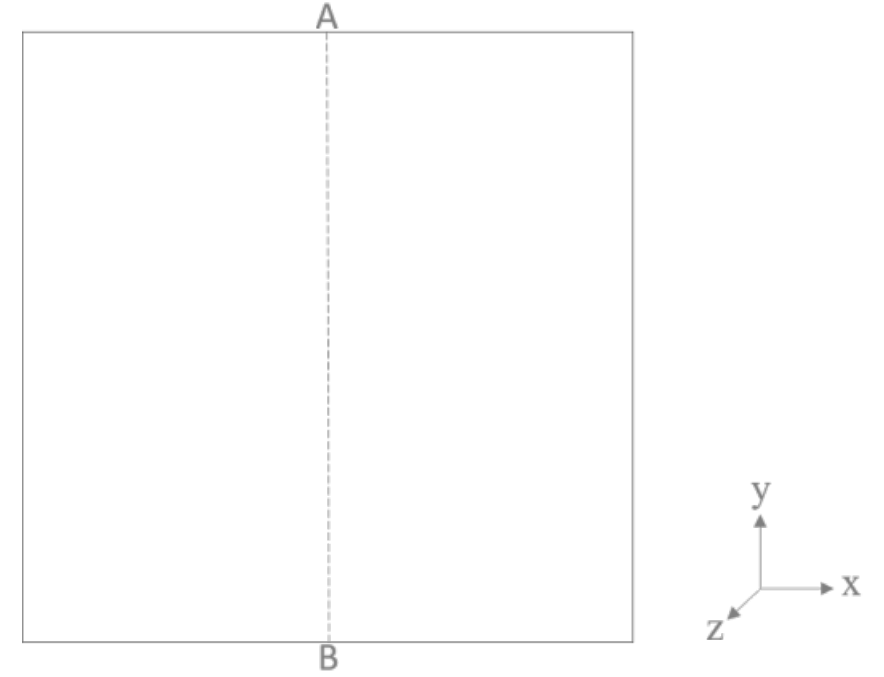
\includegraphics[width=200pt]{images/fig-eg-surf-deformer-1}
    \caption{Configuração inicial da superfície a ser deformada.~\cite{Muller}}\label{fig-eg-surf-deformer-1}
  \end{center}
\end{figure}


\begin{figure} [H]
  \begin{center}
    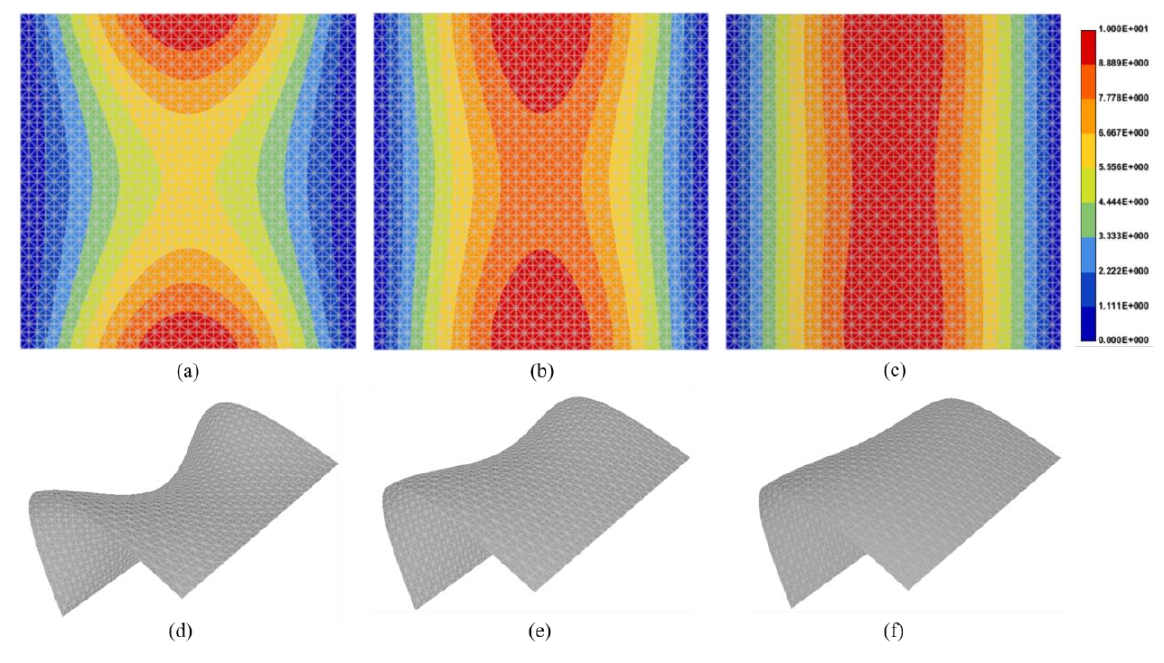
\includegraphics[width=\textwidth]{images/fig-eg-surf-deformer-2}
    \caption{Configuração deformada da superfície segundo as Lagrangeanas de 2ª ordem (a,d), 4ª ordem (b,e) e 6ª ordem (c, f). As figuras (a, b e c) representam os resultados na direção $z$, escala em metros.\cite{Muller}}\label{fig-eg-surf-deformer-2}
  \end{center}
\end{figure}

A Figura~\ref{fig-eg-surf-deformer-2} deixa clara as diferenças na deformação da superfície conforme a energia minimizada. De modo específico para a deformação de superfícies geológicas onde há um viés físico atrelado, a solução que minimiza a energia de mínima variação e que, portanto, resulta na mínima variação da curvatura é a que melhor se adequa ao comportamento previsto para este tipo de simulação.

O gráfico da Figura~\ref{fig-eg-surf-deformer-3} destaca o campo de deslocamentos em $z$ sobre o segmento $\overline{AB}$ da Figura~\ref{fig-eg-surf-deformer-1} para cada um dos três tipos de deformação mencionados.

\begin{figure} [H]
  \begin{center}
    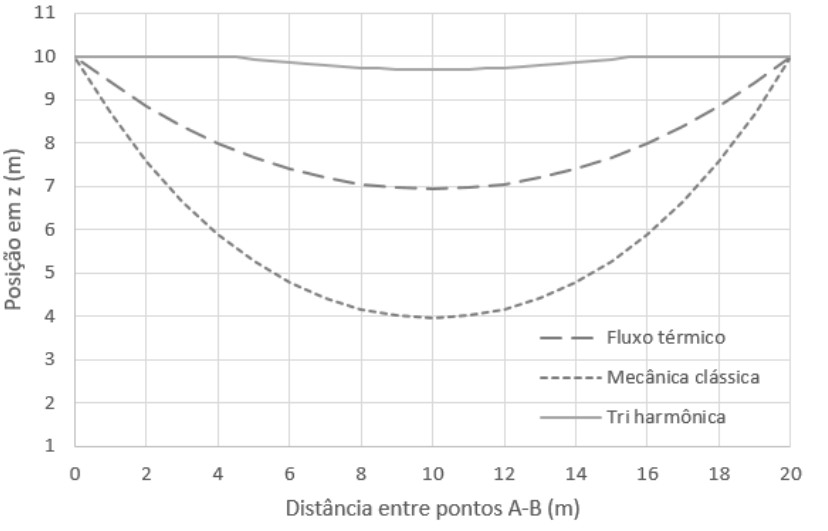
\includegraphics[width=250pt]{images/fig-eg-surf-deformer-3}
    \caption{Coordenada $z$ sobre o segmento $\overline{AB}$.\cite{Muller}}\label{fig-eg-surf-deformer-3}
  \end{center}
\end{figure}

Os procedimentos computacionais para os tipos de minimização de energia de superfície descritos nesta seção foram implementados por Müller e estão disponíveis na biblioteca \emph{MGeo Deformer}~\cite{Muller} do Sistema Recon.

\section{Preparação dos dados}
 
A metodologia mostrada anteriormente é capaz de realizar a deformação de superfície mediante conhecimento da posição inicial da mesma e também de informação de movimentação de pontos de controle, pontos estes que devem fazer parte do domínio da superfície. Desse modo, no contexto de restauração de seções no Sistema Recon, o mapeamento de superfície é obtido com a deformação desta superfície de acordo com parâmetros provenientes das seções. Em outras palavras, o mapeamento de superfície usa dados das seções como pontos de controle para se conseguir um comportamento equivalente no ambiente tridimensional. Essa é uma forma sucinta de descrever o modo como o mapeamento de superfície é feito. Nesta subseção serão apresentadas as etapas que permitem o uso do deformador de superfícies (\emph{MGeo Deformer}) com o intuito de se obter o mapeamento de superfícies.

Importante salientar que o ideal é que após a seção ter sido criada ocorra o mínimo de edição inicial nas linhas geradas. Isso é importante pois quanto melhor definida esteja a seção após o fatiamento (item~\ref{item-section-creation}), mais coerente com as superfícies tridimensionais estará o modelo como um todo. Edições nas linhas são comuns de acontecerem para que seja possível realizar a restauração da seção, entretanto, em caso de edições maiores ocorrerá o descasamento entre seção e superfícies e, nesta etapa, poderão haver incongruências.

\subsection{\textit{LMModels}}\label{lmmodels-surface-map}

O objetivo desta subseção é mostrar como obter informação de deslocamento dos horizontes entre etapas de restauração de uma seção geológica a partir de \textit{LMModels}. O deslocamento de pontos de horizonte é o dado principal vindo das seções para o mapeamento de deformações de horizontes, uma vez que as seções geológicas são cortes transversais planos de um conjunto de superfícies tridimensionais.

Como já visto, as \textit{LMModels} são linhas de mapeamento da seção baseadas em entidades geológicas. Estas linhas acompanham a movimentação tectônica na seção durante a restauração. Para esta etapa do trabalho, considera-se apenas as \textit{LMModels} de horizonte, ou seja, aquelas que tem como origem uma linha de horizonte, como as mostradas na Figura~\ref{fig-lmmodel-example}.

A movimentação tectônica da seção pode ser mensurada como uma diferença entre uma e outra etapa de restauração, mais especificamente, a distância entre os pontos de \textit{LMModels} correspondentes entre a etapa atual e a próxima.

A \textit{LMModel} em si não possui pontos geométricos, ela armazena apenas os índices dos nós do contorno da malha na extensão correspondente a uma linha de horizonte (Figura~\ref{fig-lmm-mesh-boundary}). Dessa forma, entre um cenário e outro da mesma seção, pode ocorrer uma edição na malha que pode alterar os nós do contorno e assim alterando o conjunto de índices que formam a \textit{LMModel}.

\begin{figure} [H]
  \begin{center}
    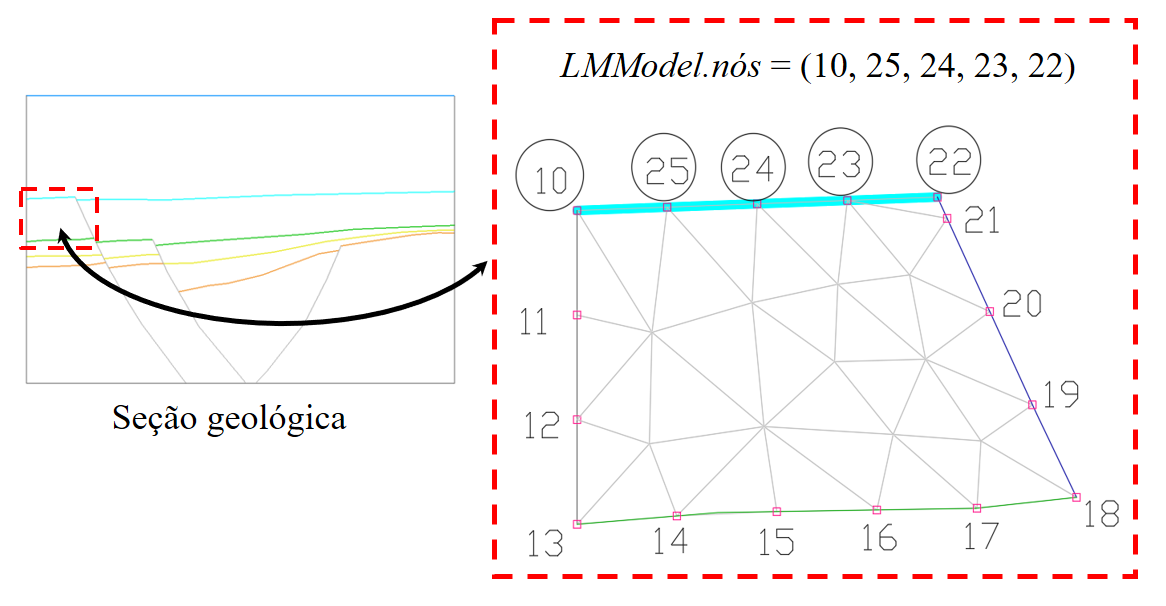
\includegraphics[width=310pt]{images/fig-lmm-mesh-boundary}
    \caption{Índices de nós que compõem uma parte de \textit{LMModels}.}\label{fig-lmm-mesh-boundary}
  \end{center}
\end{figure}

Para que se possa estabelecer uma relação direta de deslocamento entre pontos de uma \textit{LMModel} para diferentes cenários é necessário que se faça uma interpolação entre as malhas envolvidas. Esta ação serve para assegurar que se tenha um mesmo número de pontos formando a \textit{LMModel} correspondente ao longo da restauração de uma seção.

Para exemplificar melhor esse problema, considere a seção geológica da Figura~\ref{fig-lmm-interp1} (a) que destaca os pontos que formam a \textit{LMModel} do horizonte A (do topo). Considera-se que na etapa seguinte (cenário 2), houve uma transformação e uma edição na malha, com isso a \textit{LMModel} correspondente teve diminuição no número de pontos, como mostra a Figura~\ref{fig-lmm-interp1} (b).

\begin{figure} [H]
  \begin{center}
    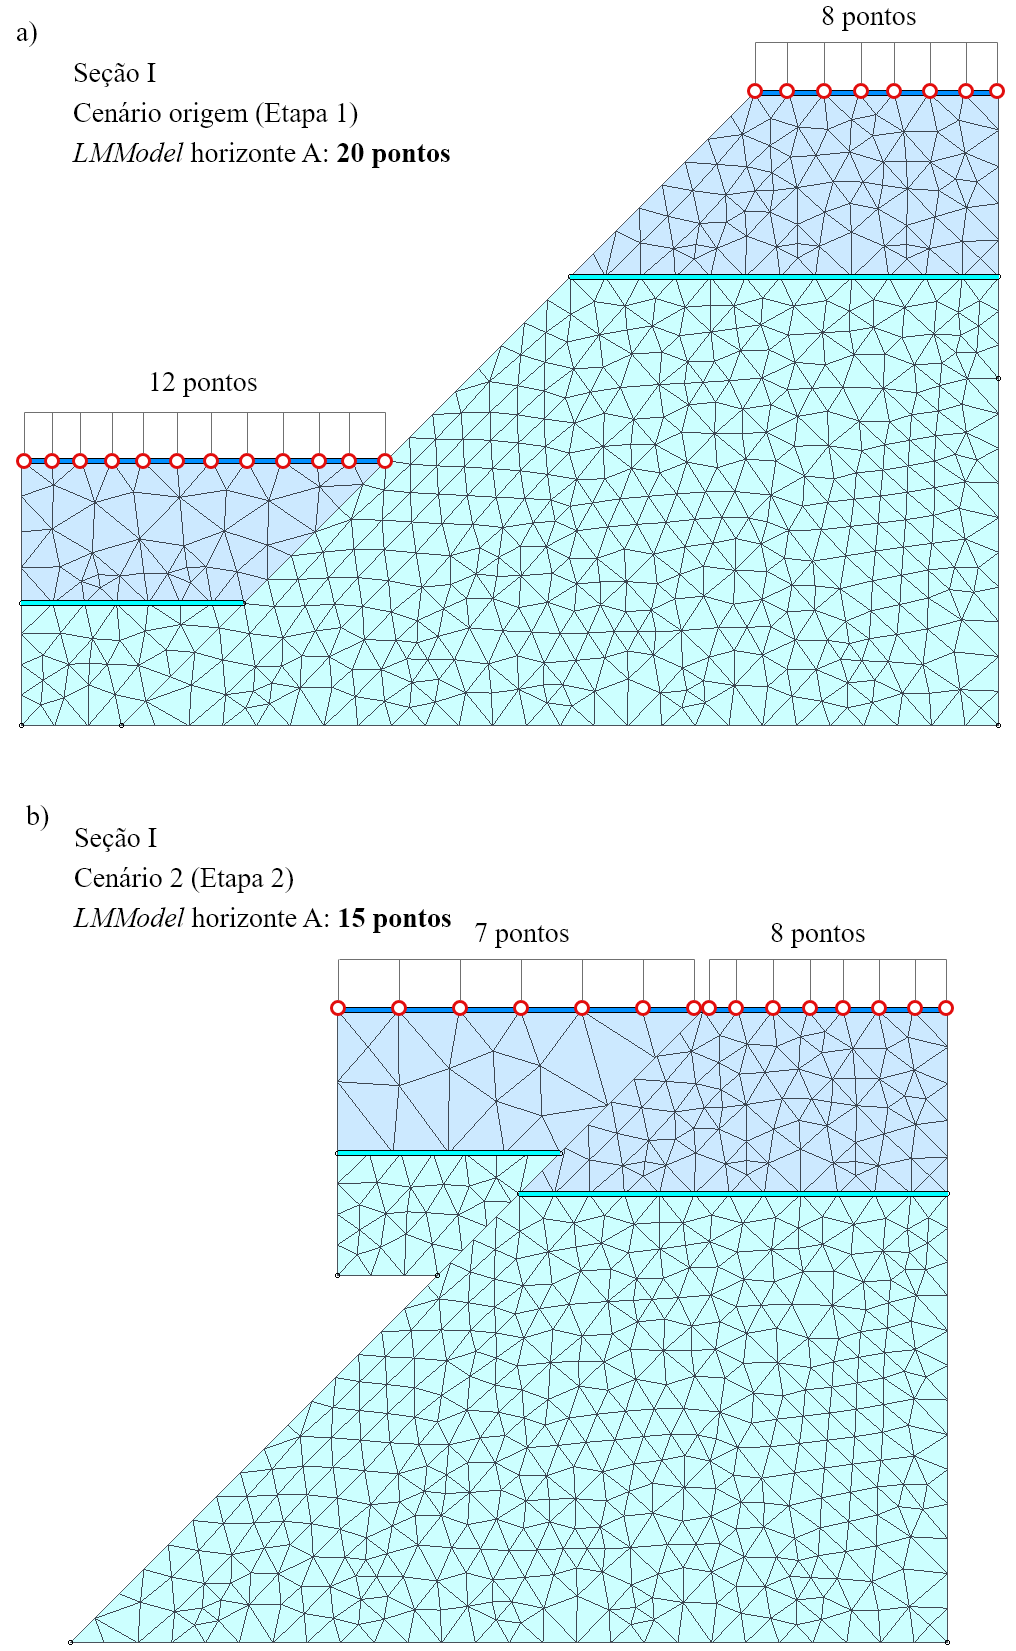
\includegraphics[width=300pt]{images/fig-lmm-interp1}
    \caption{\textit{LMModel} no cenário origem e cenário 2 com diferente número de pontos.}\label{fig-lmm-interp1}
  \end{center}
\end{figure}

Para que seja feito o cálculo de deslocamento entre as \textit{LMModels} destes cenários é necessário uma interpolação entre as malhas, como já dito. Essa interpolação fornece os pontos no cenário 2 que correspondem àqueles da \textit{LMModel} no cenário origem e assim ter dados para encontrar informações de deslocamento de uma etapa a outra.

Convencionou-se neste trabalho que a obtenção dos pontos de \textit{LMModels} toma como base para interpolação aquela criada no cenário origem, já que é um cenário mais restrito para edições após o início da restauração. Além disso, os pontos das \emph{LMModels} do cenário origem são usados com restrição para o \emph{remesh} da malha de superfície (item~\ref{surface-remesh}). Um esquema ilustrativo é visto na Figura~\ref{fig-lmm-interp2}.

\begin{figure} [H]
  \begin{center}
    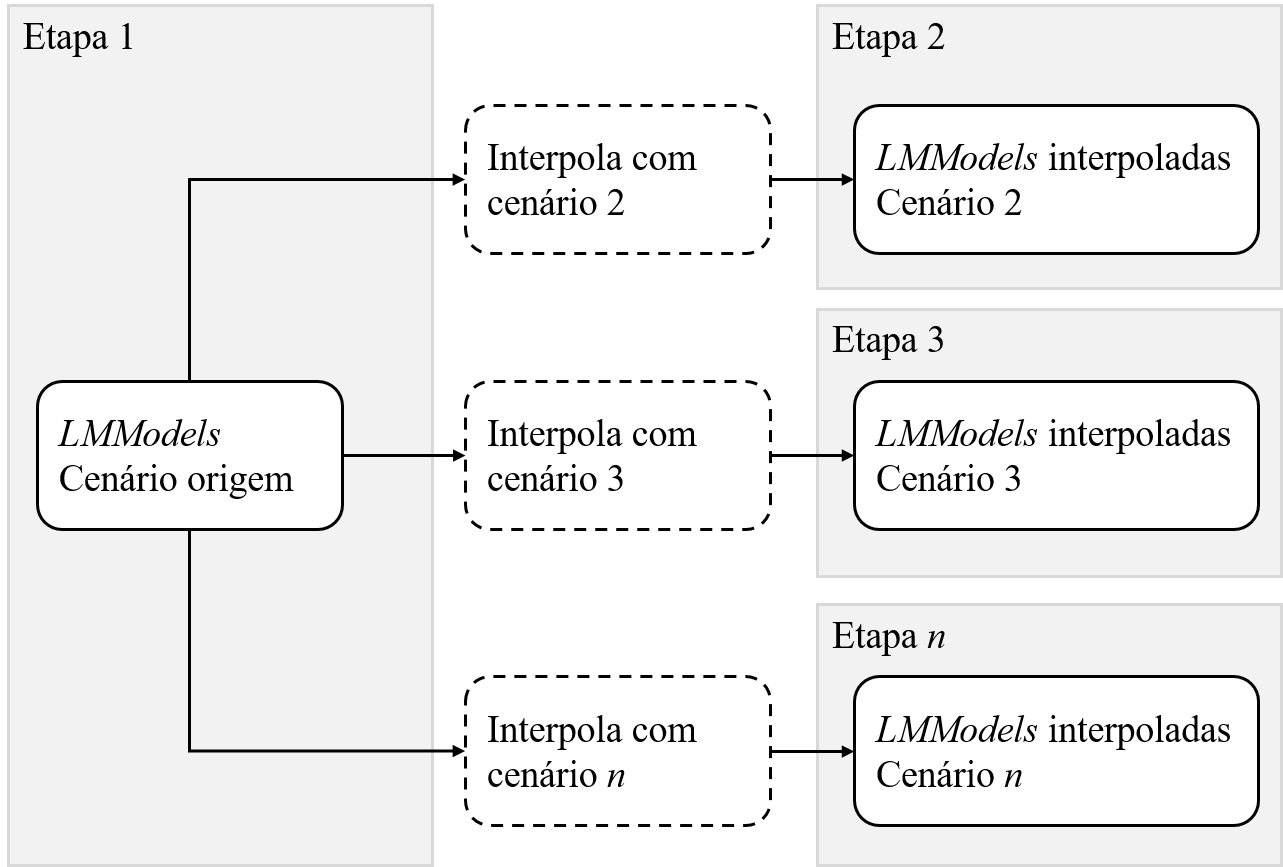
\includegraphics[width=350pt]{images/fig-lmm-interp2}
    \caption{Esquema de como obter número igual de pontos de \textit{LMModels} em diferentes cenários}\label{fig-lmm-interp2}
  \end{center}
\end{figure}

Ao se repetir esta ação para todas as seções que compõem o modelo, é possível criar uma estrutura de dados multidimensional com todos os pontos geométricos que formam as \textit{LMModels} a fim de facilitar o uso dessas informações. De maneira sucinta, esta estrutura é apresentada na Figura~\ref{fig-lmm-data-structure} como sendo análoga a uma matriz de 3 dimensões onde cada elemento é um conjunto de dois pontos cartesianos\footnote{os pontos nas malhas da seção estão em coordenadas bidimensionais, no entanto, ao criar esta estrutura de dados, todos os pontos são convertidos para coordenadas espaciais \textit{x}, \textit{y} e \textit{z} com base nas coordenadas UTM onde a seção se localiza.} e um dado booleano que indica se houve movimentação quando a diferença entre os pontos \textit{current} e \textit{next} é maior que uma dada tolerância.

\begin{figure} [H]
  \begin{center}
    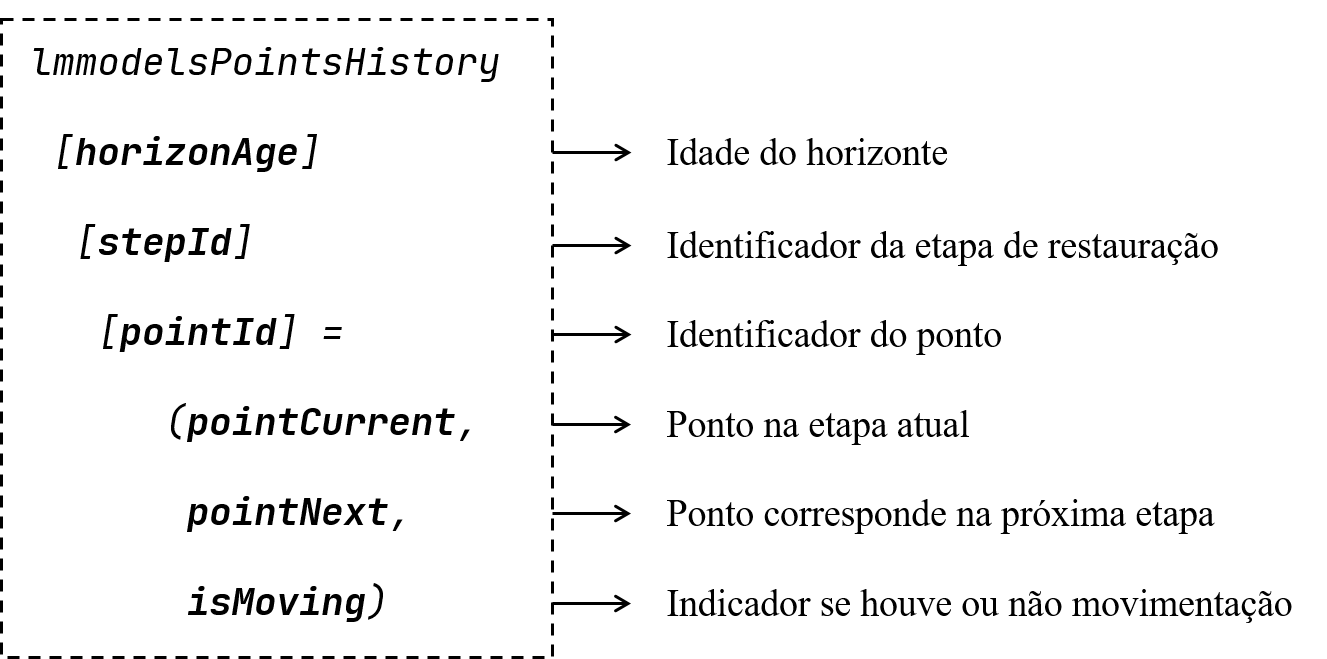
\includegraphics[width=350pt]{images/fig-lmm-data-structure}
    \caption{Estrutura de dados que armazena os pontos das \textit{LMModels} do modelo.}\label{fig-lmm-data-structure}
  \end{center}
\end{figure}

Importante ressaltar que é preciso ter o modelo já com todas as seções restauradas, uma vez que qualquer edição posterior nas seções, acarretará na necessidade de recriar a estrutura de dados de \textit{LMModels}.

\subsection{\textit{Remesh} da superfície}\label{surface-remesh}

No item~\ref{surface-mapping-metodology} foi apontada a necessidade de haver pontos de controle pertencentes à superfície, pontos estes que precisam ter sua posição final conhecida. Uma parte destes pontos de controle são as \textit{LMModels}, ou melhor, os pontos que representam o histórico de movimentação das \textit{LMModels}.

A interseção de um plano transversal a um conjunto de superfícies geológicas tridimensionais é o que produz a seção geológica, onde cada linha de horizonte é a representação de uma parte da superfície no plano bidimensional. Não por acaso, as \textit{LMModels} são mapeamentos dessas linhas de horizonte e, portanto, também mapeiam a superfície. No entanto, os pontos que formam a \textit{LMModel} foram gerados com base nas malhas de triângulos da seção e não possuem qualquer relação com os pontos que estão na superfície.

Com a finalidade de resolver esse problema é apresentado nesta subseção a necessidade de um \textit{remesh} (regeração da malha) que forma a superfície, cujo objetivo é produzir uma nova malha que contenha os pontos que formam as \textit{LMModels} das seções geológicas.

O \textit{remesh} é realizado com auxílio do algoritmo de regeração de malhas de superfícies considerando curvaturas proposto por Miranda \textit{et al.}~\cite{Miranda}. Os dados de entrada são as linhas de borda da superfície, uma malha de suporte representada por três funções generalizadas, criadas a partir da malha de suporte e um conjunto de pontos de restrição no domínio da superfície que, após o \textit{remesh} deverão fazer parte da malha.

As funções generalizadas são a maneira como a malha de suporte é representada e são apresentadas a seguir, de forma sucinta:

\renewcommand{\labelitemi}{•}
\begin{itemize}
  \item 1ª função: recebe um ponto da superfície como entrada e devolve o tamanho característico da aresta de um triângulo equilátero ideal na posição desse ponto. O cálculo desse tamanho envolve o uso de uma estrutura de dados \textit{octree}\footnote{Uma estrutura de árvore onde cada nó pode possuir oito filhos e representa a subdivisão do espaço em oito octantes~\cite{Donald}.} que fornece um refinamento de tamanho de acordo com a curvatura da superfície.
  \item 2ª função: calcula o ponto ideal que irá formar um novo triângulo de acordo com uma dada aresta no processo de contração de contorno de geração da malha. Além da aresta, são passados à função a altura do triângulo e um vetor unitário na direção perpendicular à aresta que será usado para definir o plano de interseção com a superfície e assim encontrar o ponto ideal.
  \item 3ª função: usada para melhoria na malha após a suavização. Recebe um ponto qualquer e retorna o ponto mais próximo pertencente à malha da superfície de suporte. Com a suavização, alguns nós mudam de lugar e podem acabar fora da superfície, ocorrendo isso, esta terceira função é utilizada para trazer de volta os pontos distantes. 
\end{itemize}

O algoritmo utiliza avanço de fronteira na primeira fase e faz uso da 1ª e 2ª funções para determinar a primeira versão da nova malha. Após isso começa a etapa de melhoria com suavização e em paralelo, o uso da 3ª função~\cite{Miranda}. O resultado final é uma malha com mais elementos em regiões de alta curvatura, como mostra a Figura~\ref{fig-remesh} onde as imagens (a) e (b) são as superfícies de suporte e as imagens (c) e (d) suas versões regeradas, respectivamente.

\begin{figure} [H]
  \begin{center}
    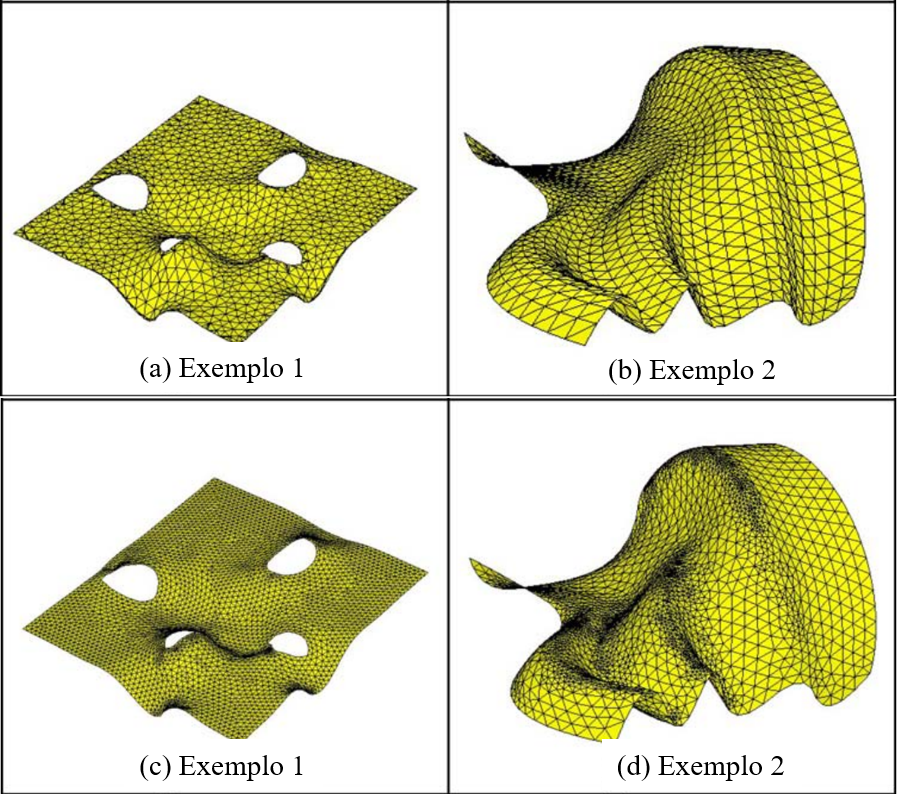
\includegraphics[width=350pt]{images/fig-remesh}
    \caption{Exemplo de resultado obtido com algoritmo de \textit{remesh}~\cite{Miranda}.}\label{fig-remesh}
  \end{center}
\end{figure}

Os pontos de restrição usados para a regeração da malha de superfície são as \textit{LMModels} da seção, portanto, passam a ser os pontos de controle da superfície geológica. Uma vez que os pontos que formam as \textit{LMModels} são todos iguais em número, pois tomam o cenário origem da \textit{EtapaMS} inicial e são interpolações com os cenários seguintes, o \textit{remesh} pode ser feito nesta \textit{EtapaMS} inicial e essa malha ser mantida para todo o restante do processo.

De uma \textit{EtapaMS} à outra, com as \textit{LMModels}, é possível ter o deslocamento das linhas de horizontes, por exemplo. Sendo os pontos das \textit{LMModels} nós da malha da superfície, esses nós passam a ter informação de posição final definida. Sendo assim, já seria possível realizar a deformação da superfície conforme metodologia já apresentada, pois o principal requisito está satisfeito. No entanto, se tratando do mapeamento de uma superfície que, num modelo geológico de multisseções, precisa estar coerente com o que ocorre nas seções, mais algumas restrições precisam ser impostas conforme descrito nas subseções a seguir.

\subsection{Definição das bordas origem/destino}

Na restauração de seções um dos principais objetivos é a eliminação do rejeito de falha, principalmente se tratando de modelos de tectônica distensiva onde há a presença de blocos divididos por essas falhas~\cite{Santi}. Nestes modelos, geralmente se quer movimentar um bloco sobre uma linha de falha até um certo ponto, de modo que a camada do topo esteja alinhada com a sua correspondente no bloco vizinho. A Figura~\ref{fig-section-horizon-restored} mostra uma seção com um horizonte restaurado com o uso da transformação \quotes{move sobre falha}.

\begin{figure} [H]
  \begin{center}
    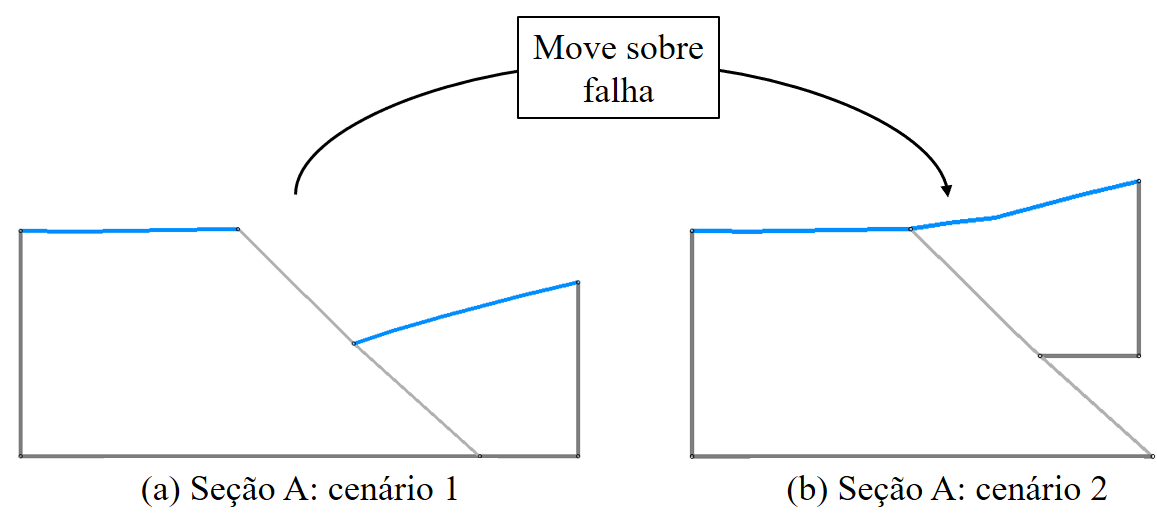
\includegraphics[width=350pt]{images/fig-section-horizon-restored}
    \caption{Restauração de horizonte em uma seção geológica através de uma transformação.}\label{fig-section-horizon-restored}
  \end{center}
\end{figure}

Esta ação de movimentar uma porção da seção até um certo limite é um comportamento necessário no mapeamento de superfícies, isto é, o mapeamento de superfícies precisa respeitar um limite de movimentação análogo àquele adotado na seção.

Em geral, no uso do Sistema Recon, uma \textit{EtapaMS} representa um marco geológico ocorrido em todas as seções do modelo simultaneamente. O que para este trabalho convencionou-se que seja uma restauração do rejeito de uma falha ou uma descompactação de topo restaurado. Logo, para o mapeamento de superfícies, é necessário que cada \textit{EtapaMS} represente a restauração de uma falha (ou descompactação) ocorrida ao mesmo tempo em todas seções onde tal falha atravesse. Pois, como nas seções, as superfícies de horizontes também estão com as falhas cruzando seu domínio, como mostra a Figura~\ref{fig-surfaces-horizon-faults}.

\begin{figure} [H]
  \begin{center}
    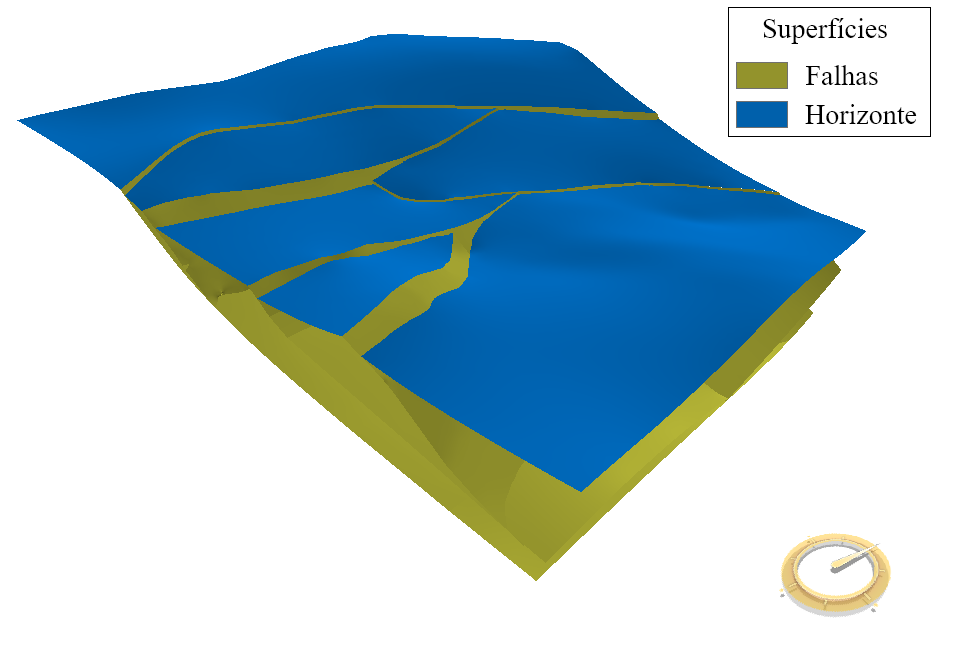
\includegraphics[width=310pt]{images/fig-surfaces-horizon-faults}
    \caption{Vista 3D de uma superfície de horizonte atravessada por várias superfícies de falhas.}\label{fig-surfaces-horizon-faults}
  \end{center}
\end{figure}

Como forma de definir limites de movimentação na deformação da superfície, pode-se indicar bordas de origem e destino da superficie. Esse é um procedimento análogo à movimentação de bloco ocorrida nas seções ao longo de uma falha. Essa indicação servirá ainda para auxiliar na definição da direção de movimentação das partes envolvidas em uma dada \textit{EtapaMS} na deformação da superfície.

Esse mapeamento de superfície é feito passo a passo conforme o número de \textit{EtapasMS} do modelo. Com a \textit{EtapaMS} vem a informação de qual falha está sendo restaurada\footnote{Para o caso de descompactação, a etapa de selecionar bordas não é necessária.}, com isso é necessário selecionar e marcar as bordas da superfície na região da falha para assim guiar a direção e o limite de movimentação durante a deformação da mesma.

O processo em mais detalhes pode ser explicado com o auxílio do exemplo de um modelo geológico simplificado, mostrado na Figura~\ref{fig-select-borders-1}, onde há uma superfície de horizonte, uma falha, 3 seções transversais e cuja \textit{EtapaMS} corrente é a de restauração dessa falha.

\begin{figure} [H]
  \begin{center}
    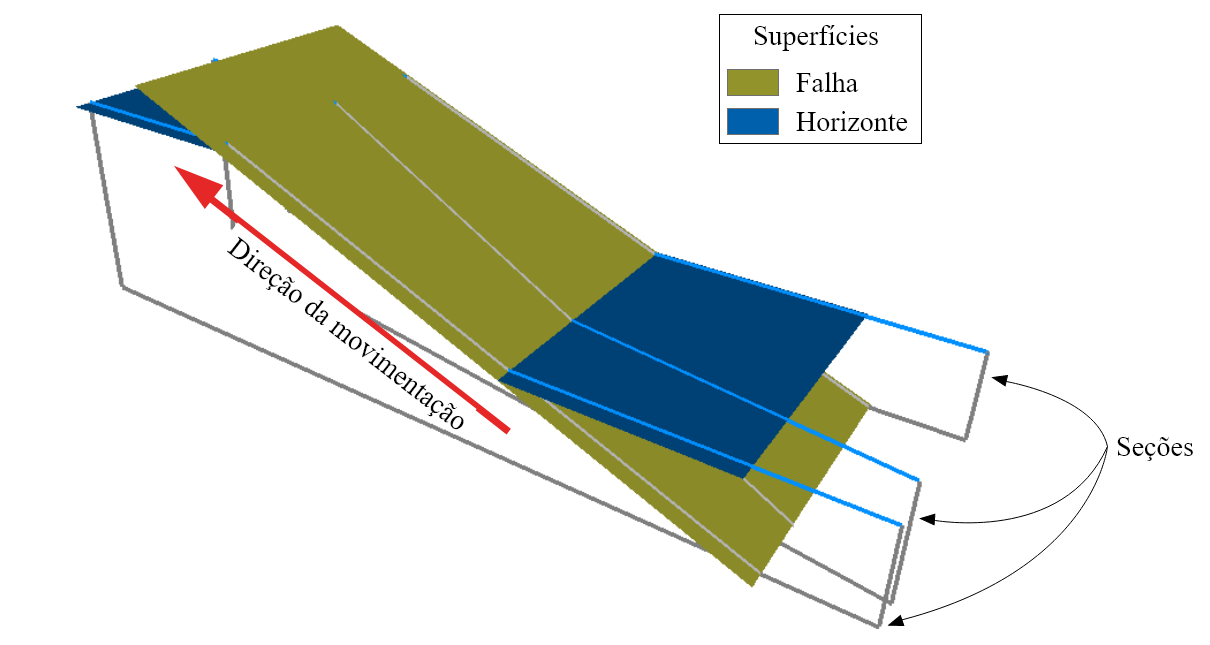
\includegraphics[width=350pt]{images/fig-select-borders-1}
    \caption{Modelo geológico tridimensional simplificado.}\label{fig-select-borders-1}
  \end{center}
\end{figure}

Neste caso, tal qual ocorre nas seções, o pedaço de superfície de horizonte à direita na imagem é que deve se movimentar e ir de encontro à parte que está do lado esquerdo. Logo, o pedaço à direita possui a borda de origem e o da esquerda, a borda de destino, como mostra a Figura~\ref{fig-select-borders-2}.

\begin{figure} [H]
  \begin{center}
    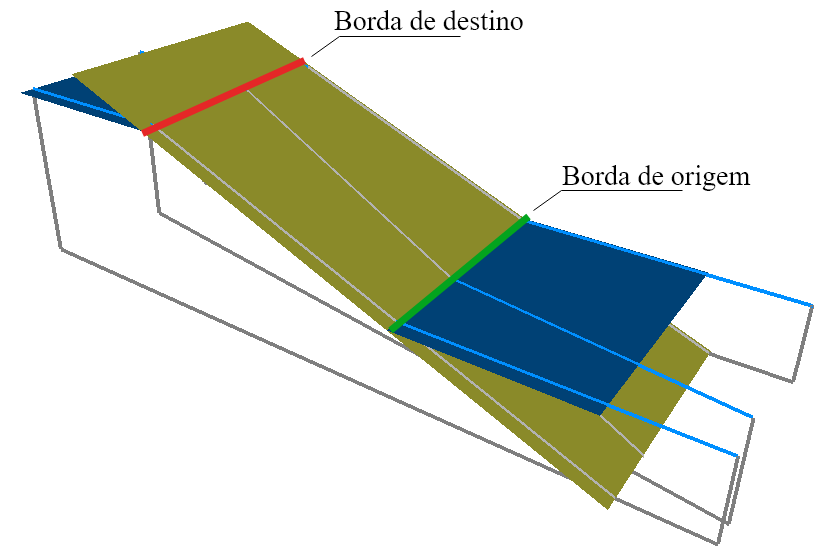
\includegraphics[width=300pt]{images/fig-select-borders-2}
    \caption{Indicação da localização das curvas origem e destino}\label{fig-select-borders-2}
  \end{center}
\end{figure}

A partir dessa marcação, que na prática ocorre nos pontos do contorno da malha da superfície, são calculados os vetores direção de cada ponto da borda de origem que deverão se deslocar até interceptar a linha poligonal formada pelos pontos da curva de destino. Esse algoritmo, se baseia na direção das seções no plano \textit{xy}, como numa vista de mapa. Observa-se pela Figura~\ref{fig-select-borders-3}, com vista em mapa, que nesse exemplo a seção do meio (seção S2) está inclinada em relação às outras seções que são paralelas entre si.

\begin{figure} [H]
  \begin{center}
    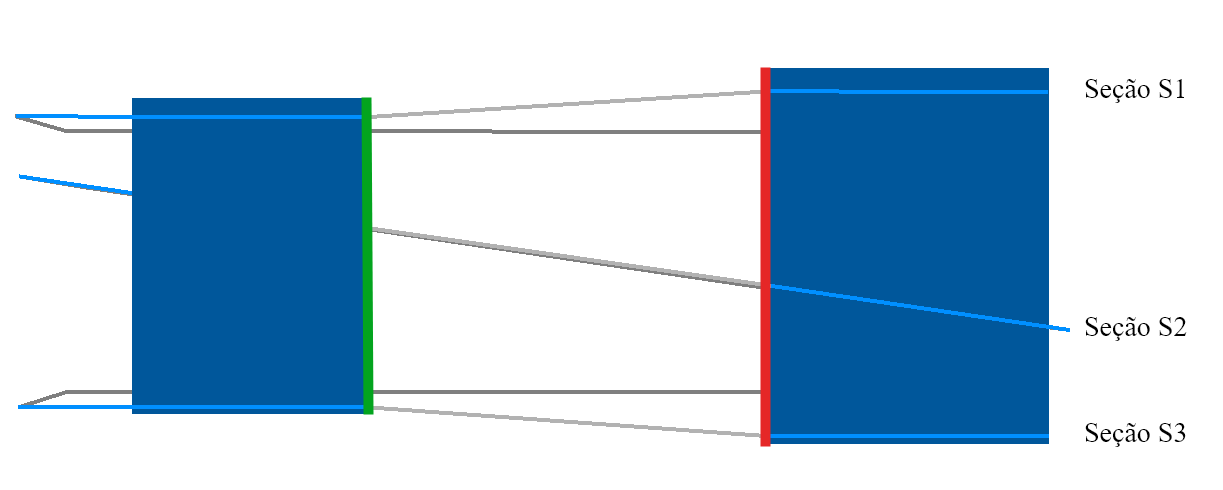
\includegraphics[width=350pt]{images/fig-select-borders-3}
    \caption{Vista de mapa do modelo para evidenciar a direção das seções.}\label{fig-select-borders-3}
  \end{center}
\end{figure}

A fim de dar mais detalhes sobre como o algoritmo de cálculo das direções funciona, considere a ilustração na Figura~\ref{fig-select-borders-4} com base nas seções e nas bordas de origem e destino desprezando o eixo \textit{z}:

\begin{figure} [H]
  \begin{center}
    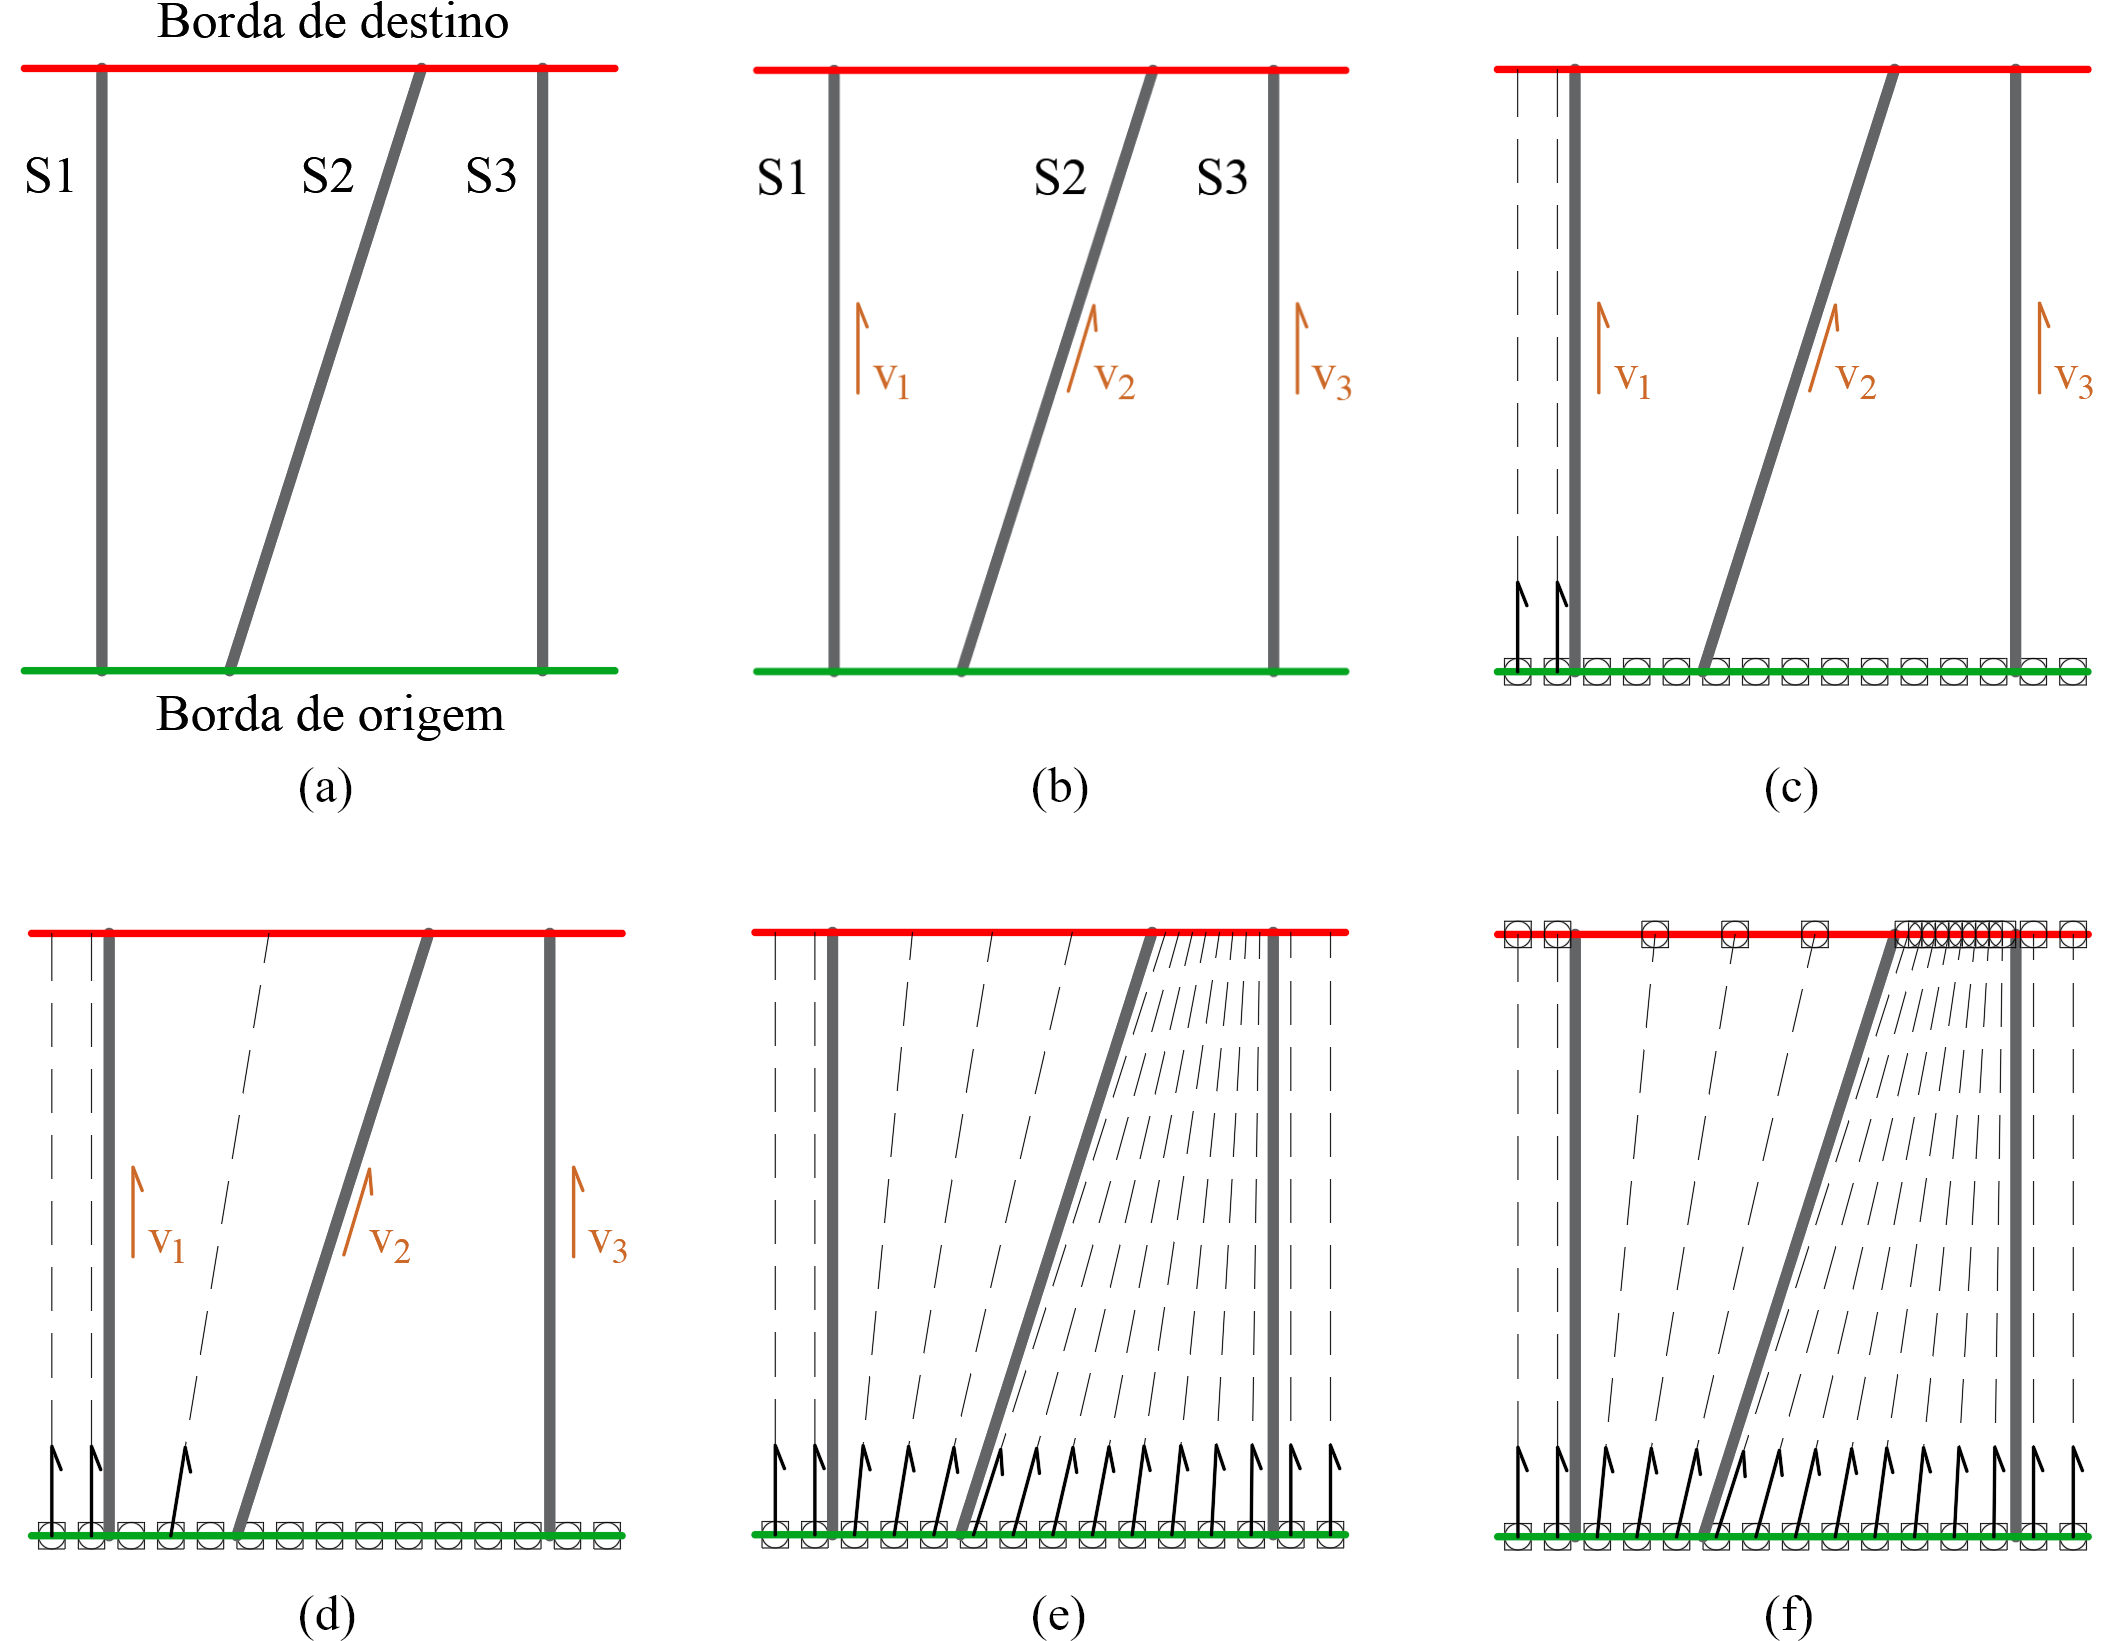
\includegraphics[width=370pt]{images/fig-select-borders-4}
    \caption{Procedimento para cálculo da direção dos pontos da borda de origem para a borda de destino.}\label{fig-select-borders-4}
  \end{center}
\end{figure}

Na Figura~\ref{fig-select-borders-4}-a estão representadas as bordas origem e destino e também as seções geológicas que cortam essas bordas. A primeira parte do procedimento (Figura~\ref{fig-select-borders-4}-b) consiste em calcular o vetor unitário que tem a mesma inclinação das seções. Isso é feito com dados dos pontos de interseção da seção com as superfícies de falha na região das bordas. Com as direções das seções definidas, se inicia o cálculo da direção dos pontos da superfície na borda de origem (Figura~\ref{fig-select-borders-4}-c), cada ponto à esquerda da primeira seção recebe a mesma direção desta. Para pontos de borda que estão entre seções (Figura~\ref{fig-select-borders-4}-d), a direção é calculada como uma combinação linear das direções das seções vizinhas, com base na distância do ponto até a interseção destas seções com a borda de origem. Prossegue-se com o cálculo de todas as direções dos pontos de borda (Figura~\ref{fig-select-borders-4}-e) e assim como nos pontos à esquerda da primeira seção, os pontos que estão logo ao lado direito da última seção recebem a direção desta. Por último (Figura~\ref{fig-select-borders-4}-f), são calculados os pontos de destino dos pontos da borda de origem, com o vetor direção, é traçado uma reta até interceptar (ou não) a poligonal formada pela borda de destino, caso haja a interseção, esse ponto é salvo como destino do ponto da borda de origem.

Assim como os pontos das \textit{LMModels}, cada ponto da borda de origem que encontrar um ponto correspondente na borda de destino da superfície passa a ser um ponto de controle, pois possui uma posição final definida, que irá auxiliar na deformação da superfície ao ser executado o mapeamento.

Importante salientar que a definição das bordas origem e destino só é requerida para a superfície que está no topo do modelo pois a restrição na movimentação se baseia em unir partes do horizonte do topo, assim como ocorre nas seções.

\subsection{Definição de movimentação dos nós da superfície}

Outra característica presente na restauração de seções com falhas distensivas é que, conforme a metodologia de restauração, o bloco alto permanece parado enquanto o bloco baixo se movimenta deslizando-se pela linha de falha (Figura~\ref{fig-hang-foot-wall}).

\begin{figure} [H]
  \begin{center}
    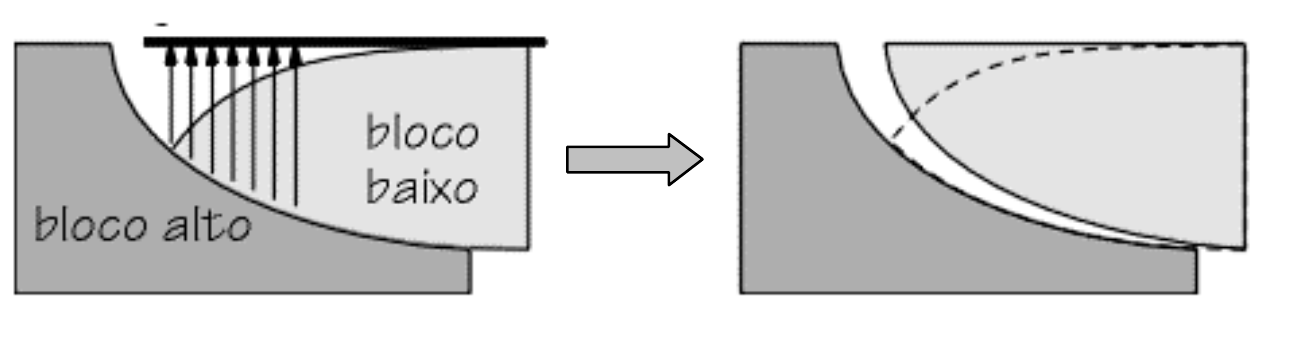
\includegraphics[width=300pt]{images/fig-hang-foot-wall}
    \caption{Movimentação do bloco baixo sobre o bloco alto.~\cite{Santi}}\label{fig-hang-foot-wall}
  \end{center}
\end{figure}

Este é um caso comum que ocorre no processo de restauração, onde quase sempre uma parte da seção se movimenta em relação a uma parte que fica imóvel. Assim como discutido na subseção anterior, este comportamento também precisa ser levado para o mapeamento de superfície a fim de manter a coerência no ambiente tridimensional, uma vez que trata-se do mesmo modelo.

Na deformação da superfície, na definição do mapeamento da mesma, é preciso indicar, a cada etapa, quais pontos da superfície irão se movimentar e quais permanecerão imóveis. De imediato, é correto afirmar que os pontos das \textit{LMModels} que possuem posição final diferente da posição inicial e também os pontos da borda de origem que têm um correspondente na borda de destino irão se movimentar. Também se pode garantir que os pontos das \textit{LMModels} que não mudam de uma \textit{EtapaMS} para outra e os pontos da borda de destino ficarão imóveis.

Todos estes pontos fazem parte da malha da superfície (após o \textit{remesh}) e são eles os primeiros a receber essa marcação de \quotes{move} ou \quotes{não move}. Para o restante dos pontos a marcação é feita com o auxílio do algoritmo de \textit{breadth-first search} (BFS) ou busca em largura~\cite{Nilsson}. Essa BFS roda sobre um grafo construído com base na malha da superfície. 

Para criar esse grafo, ocorre uma iteração por todos as arestas da malha da superfície para coleta dos índices de seus dois vértices, $v_i$ e $v_j$. Cada vértice no grafo possui uma lista de outros vértices que são seus adjacentes. Na lista do primeiro vértice $v_i$ é adicionado o segundo vértice $v_j$. Assim, no grafo, cada nó possui uma lista de seus nós adjacentes.

Com o grafo pronto é preciso identificar os primeiros a receberem uma marcação de \quotes{move} ou \quotes{não move}, sumarizando:

\renewcommand{\labelitemi}{•}
\begin{itemize}
  \item todos os nós da borda de origem são marcados como \quotes{move};
  \item todos os nós da borda de destino são marcados como \quotes{não move};
  \item Os pontos das \textit{LMModels} (que são parte da superfície) são marcados como: \quotes{move} se o correspondente na próxima \textit{EtapaMS} estiver em outra posição e \quotes{não move}, caso contrário (não há deslocamento).
\end{itemize}

A BFS é um algoritmo que realiza uma busca a partir de todos os nós do primeiro nível, daí então vai para o segundo nível que são todo os nós vizinhos do primeiro e assim por diante~\cite{Nilsson}, como mostrado na Figura~\ref{fig-bfs}, sempre visitando todos os nós do nível corrente antes de incrementar a posição na profundidade dos dados.

\begin{figure} [h]
  \begin{center}
    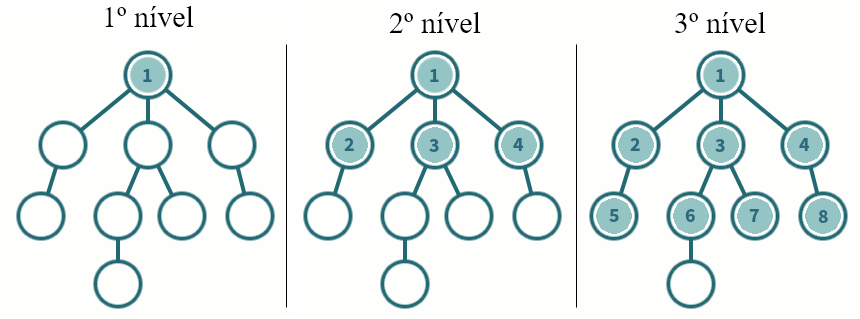
\includegraphics[width=350pt]{images/fig-bfs}
    \caption{Busca em largura ou BFS.~\cite{BFS}}\label{fig-bfs}
  \end{center}
\end{figure}

Neste caso, o primeiro nível é formado por todos os pontos inicialmente marcados, seja com \quotes{move} ou \quotes{não move}, inicia-se então a iteração com a BFS onde cada nó visitado posteriormente recebe a mesma marcação do vizinho anterior. Este laço se repete até que todos os nós da superfície tenham sido visitados.

\section{Exemplos e resultados}

Nesta seção são apresentados alguns exemplos para demonstrar o mapeamento de superfícies com base na restauração de seções. Todo o processo foi feito em uma versão experimental do Sistema Recon onde os desenvolvimentos deste trabalho têm sido implementados.

\subsection{Exemplo: modelo geológico simplificado}

Como já apresentado na Figura~\ref{fig-select-borders-1}, este é um modelo produzido manualmente que serviu para a experimentação na fase inicial do desenvolvimento deste trabalho. Ele, de forma mais completa, apresenta três seções paralelas, dois horizontes e uma falha (Figura~\ref{fig-example-1-1}). Também possui apenas uma etapa de restauração. 

\begin{figure} [H]
  \begin{center}
    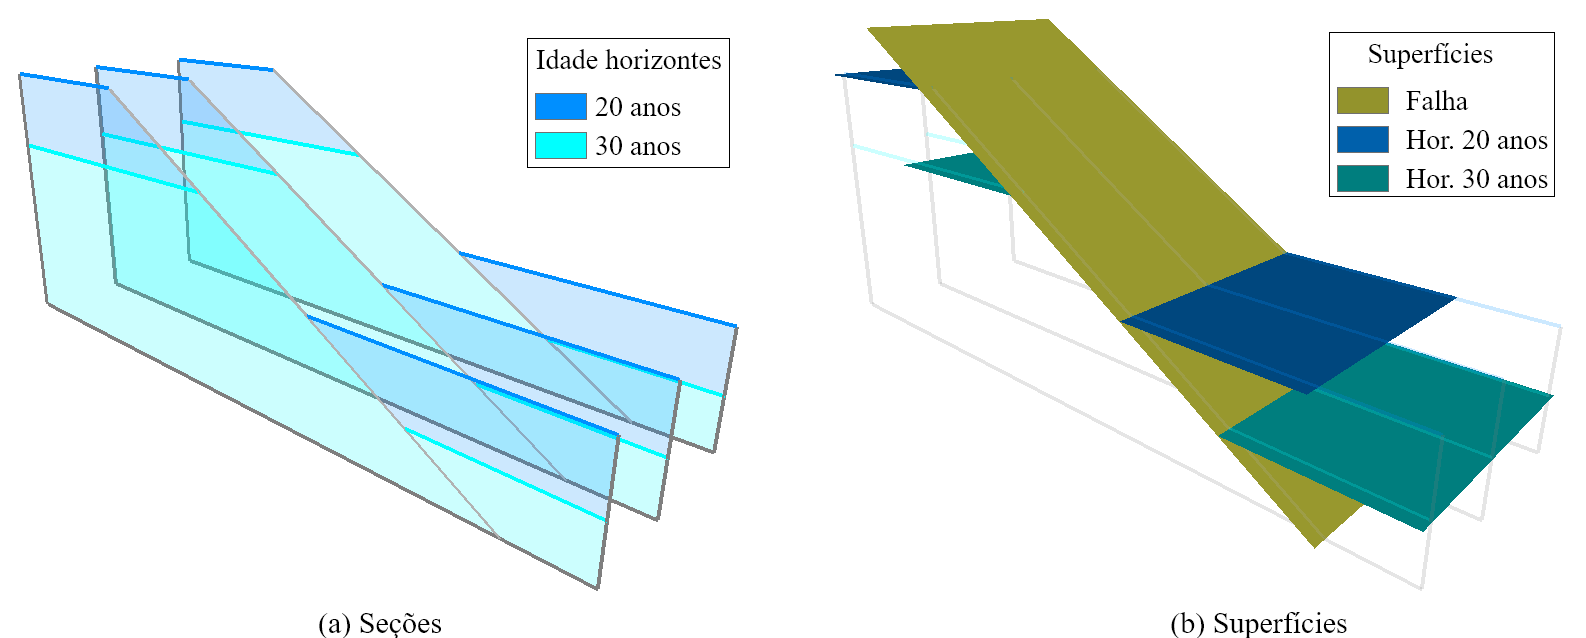
\includegraphics[width=\textwidth]{images/fig-example-1-1}
    \caption{Vista tridimensional das (a) seções e (b) superfícies do modelo simplificado.}\label{fig-example-1-1}
  \end{center}
\end{figure}

O modelo já se encontra com suas seções geológicas restauradas, com isso então pode-se começar com a criação das \textit{LMModels} e sua estrutura de dados com a forma apresentada na Figura~\ref{fig-lmm-data-structure}. A representação visual das \textit{LMModels} criadas pode ser vista na Figura~\ref{fig-example-1-2}.

\begin{figure} [h]
  \begin{center}
    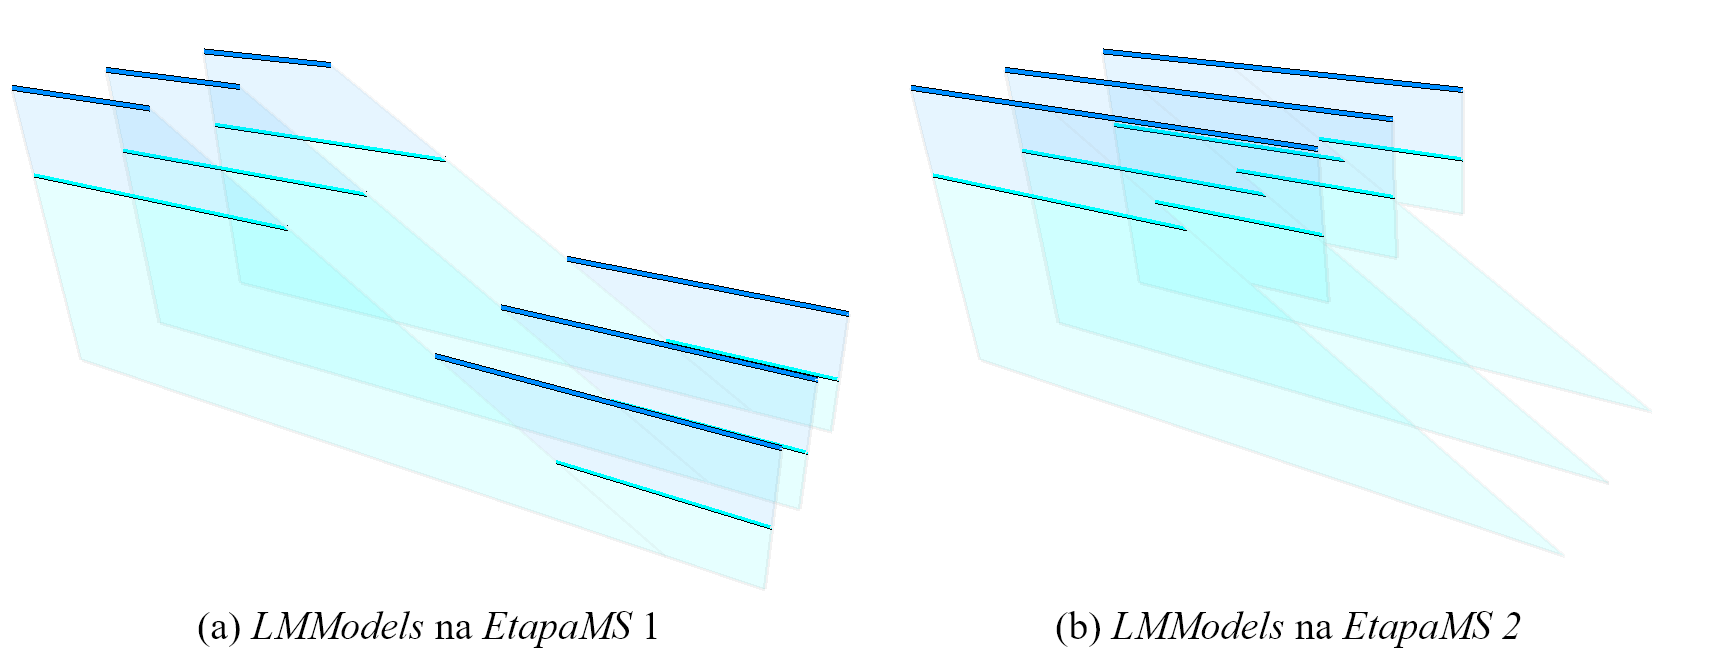
\includegraphics[width=\textwidth]{images/fig-example-1-2}
    \caption{Vista tridimensional das \textit{LMModels} nas \textit{EtapasMS} 1 e 2.}\label{fig-example-1-2}
  \end{center}
\end{figure}

Após a criação das \textit{LMModels} realiza-se o \textit{remesh} das superfícies para adicionar os pontos das \textit{LMModels} como nós da malha. A Figura~\ref{fig-example-1-3} mostra as malhas das superfícies de horizonte da parte de cima do modelo, evidenciando ainda os pontos das \textit{LMModels} que agora deverão fazer parte da malha como a imagem à direita mostra.

\begin{figure} [H]
  \begin{center}
    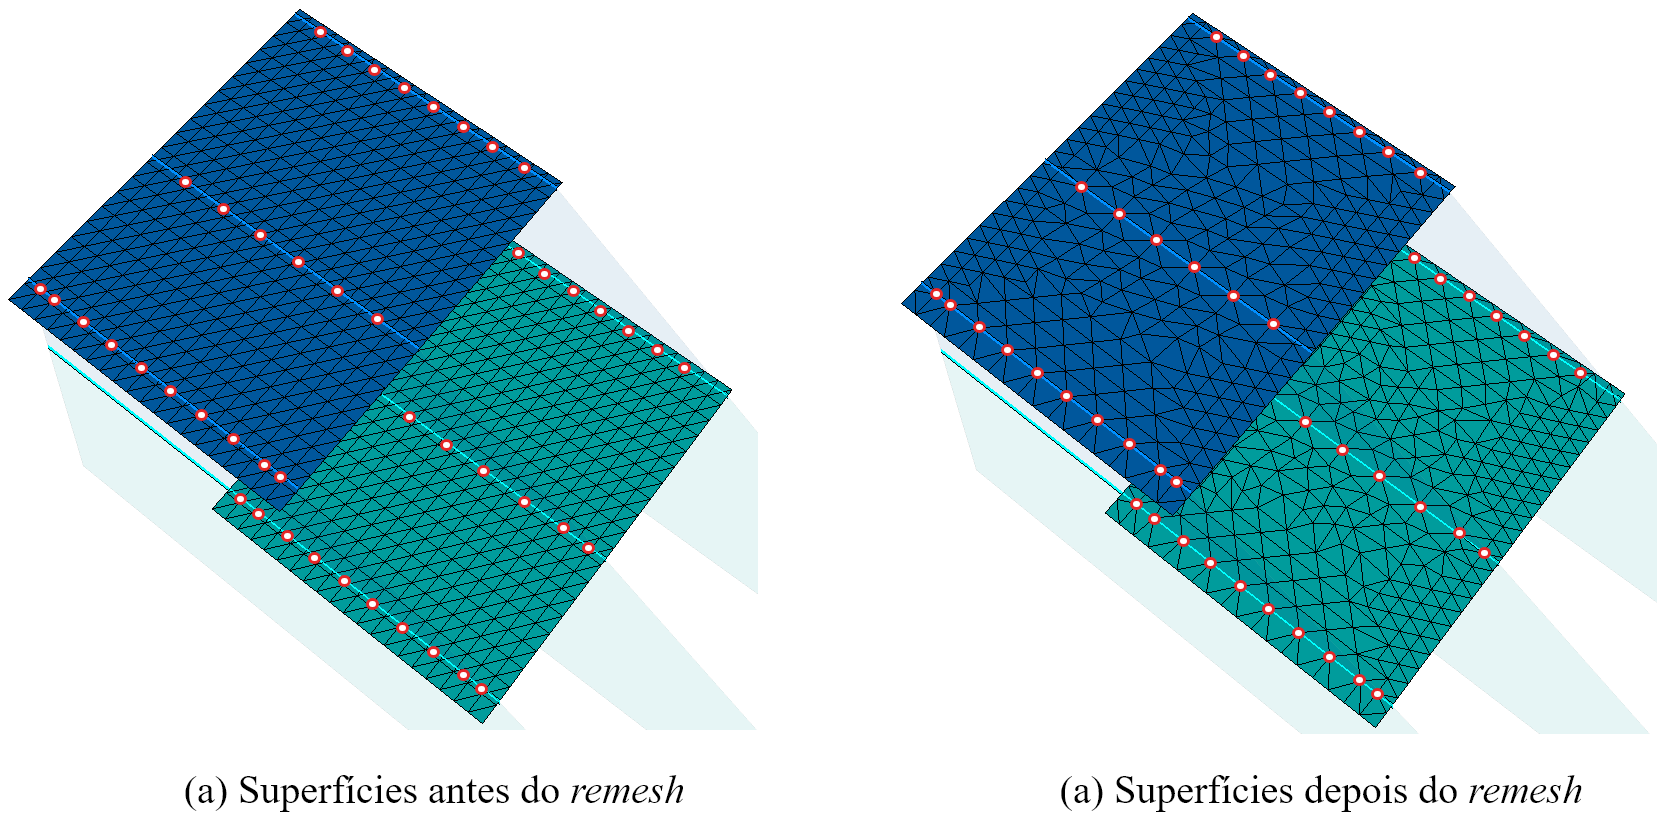
\includegraphics[width=\textwidth]{images/fig-example-1-3}
    \caption{Superfícies de horizonte antes e depois do \textit{remesh} para inclusão das \textit{LMModels} nas malhas.}\label{fig-example-1-3}
  \end{center}
\end{figure}

Logo depois do \textit{remesh}, parte-se para a definição das bordas origem e destino da superfície de horizonte do topo, que são aquelas que deverão se unir ao fim da deformação aplicada à superfície. Na Figura~\ref{fig-example-1-4} é possível notar os nós da borda dos pedaços de superfície do topo, dentre esses nós estão marcados aqueles que formam o trecho de borda de destino e origem, também sinalizados na Figura~\ref{fig-example-1-4}.

\begin{figure} [H]
  \begin{center}
    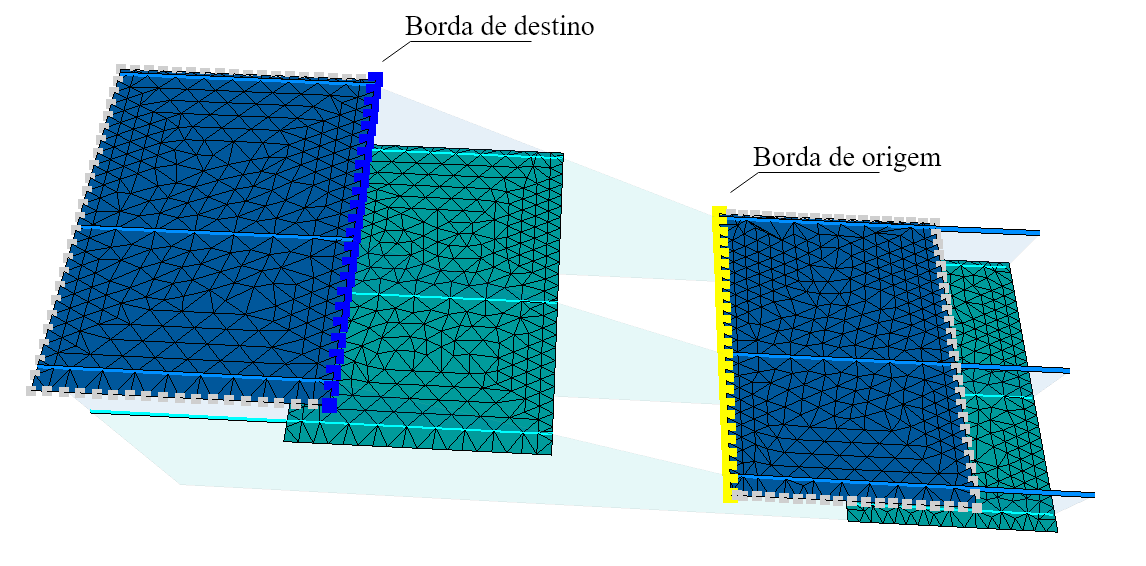
\includegraphics[width=350pt]{images/fig-example-1-4}
    \caption{Seleção das bordas de origem e destino do exemplo 1.}\label{fig-example-1-4}
  \end{center}
\end{figure}

Na etapa seguinte, calculam-se as direções dos pontos de borda e também a definição dos pontos que se movem ou não da malha da superfície. Esses dois passos são feitos após a confirmação da escolha das bordas, de forma automática. Finalmente, é chamado o algoritmo do deformador de superfícies. A próxima imagem na Figura~\ref{fig-example-1-5} mostra as superfícies deformadas segundo a restauração das seções. À direita são vistos, em destaque, os pontos da superfície que foram marcados como \quotes{move}, em verde e \quotes{não move}, em vermelho.

\begin{figure} [H]
  \begin{center}
    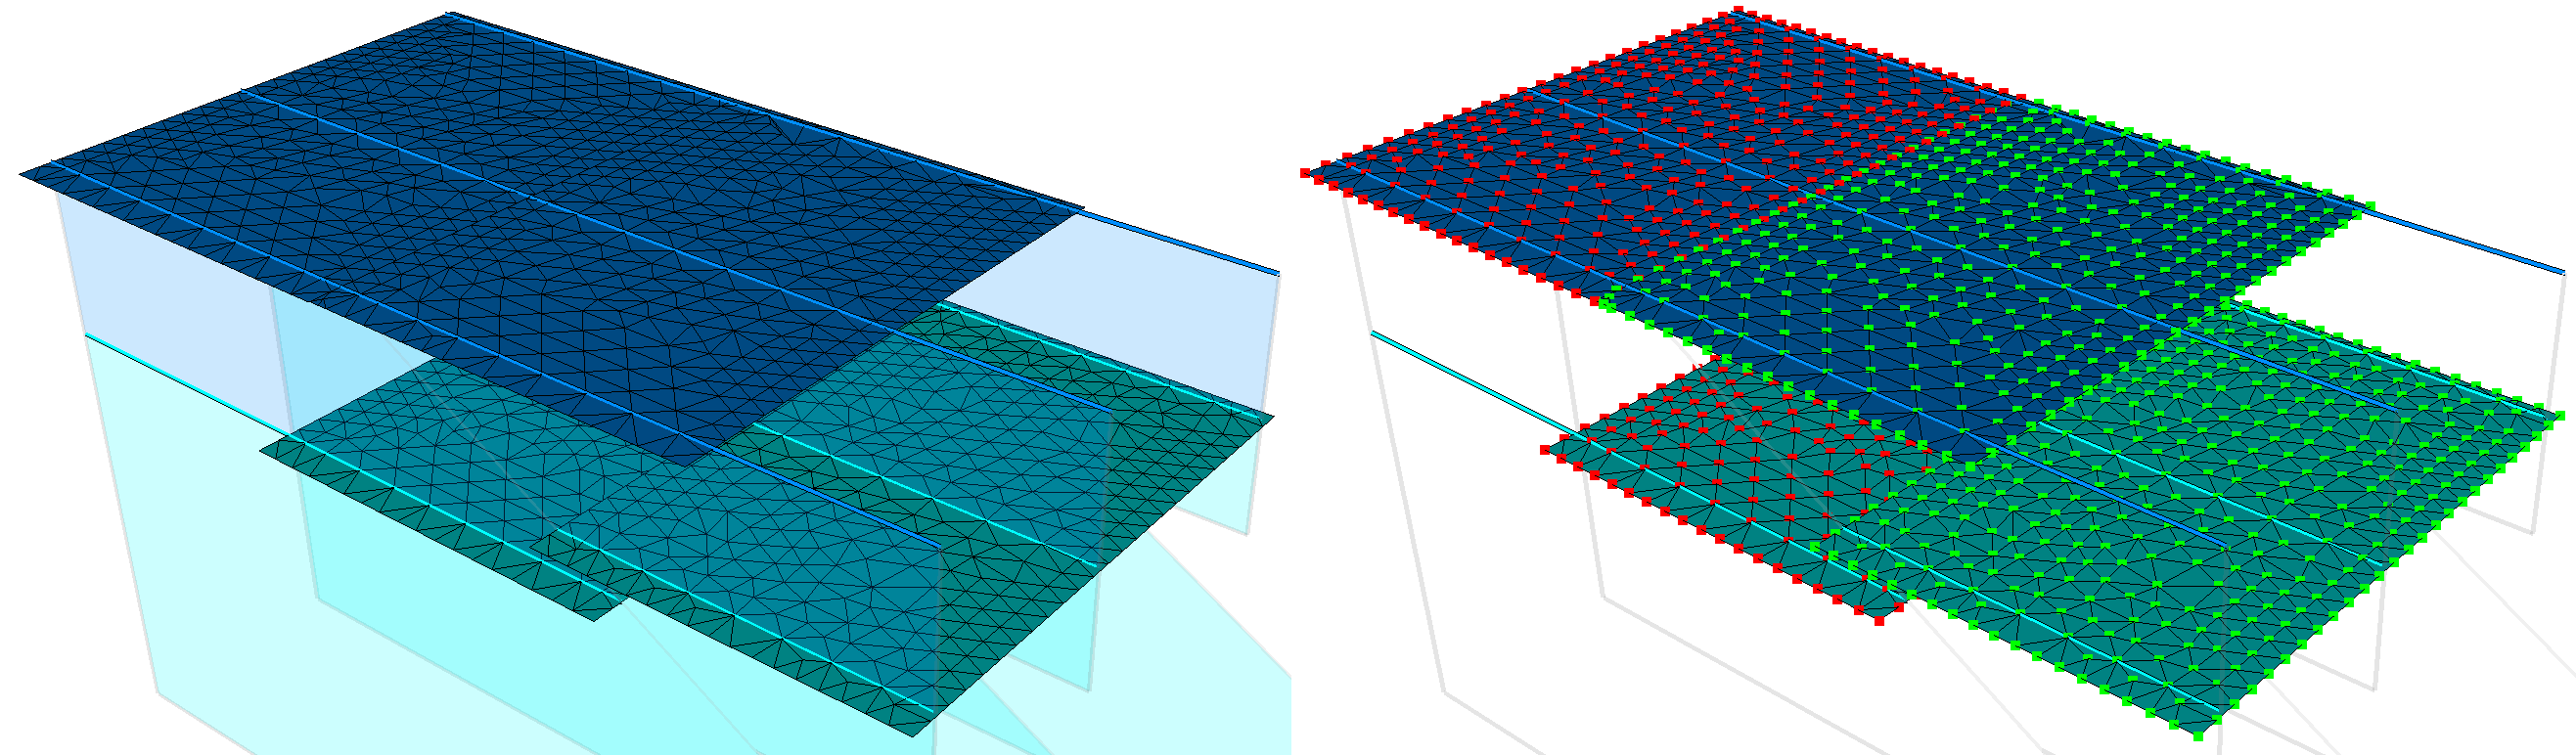
\includegraphics[width=\textwidth]{images/fig-example-1-5}
    \caption{Mapeamento de superfície do modelo de exemplo 1.}\label{fig-example-1-5}
  \end{center}
\end{figure}

O deformador de superfícies é chamado uma vez para cada superfície do modelo, no entanto, apenas a superfície do topo possui um conjunto de pontos de controle na borda próxima à falha que está sendo restaurada, ficando assim, as superfícies mais velhas sendo deformadas apenas com base na restauração das seções através das \textit{LMModels}.

\subsection{Exemplo: modelo geológico Cenpes}\label{ex-2-surf}

Este segundo exemplo utiliza um modelo geológico adaptado cedido pelo Centro de Pesquisa, Desenvolvimento e Inovação Leopoldo Américo Miguez de Mello (Cenpes/Petrobras)~\cite{Cenpes}, com dois horizontes e sete falhas com suas respectivas superfícies. No modelo foram criadas e restauradas 16 seções e conta ao todo com 14 \textit{EtapasMS}. A Figura~\ref{fig-example-2-1} mostra o modelo geológico numa vista tridimensional de cima (a) com a superfície do horizonte mais recente e (b) da superfície do horizonte mais antigo além da identificação das falhas. E a Figura~\ref{fig-example-2-2} exibe as seções geológicas numa vista tridimensional.

\begin{figure} [H]
  \begin{center}
    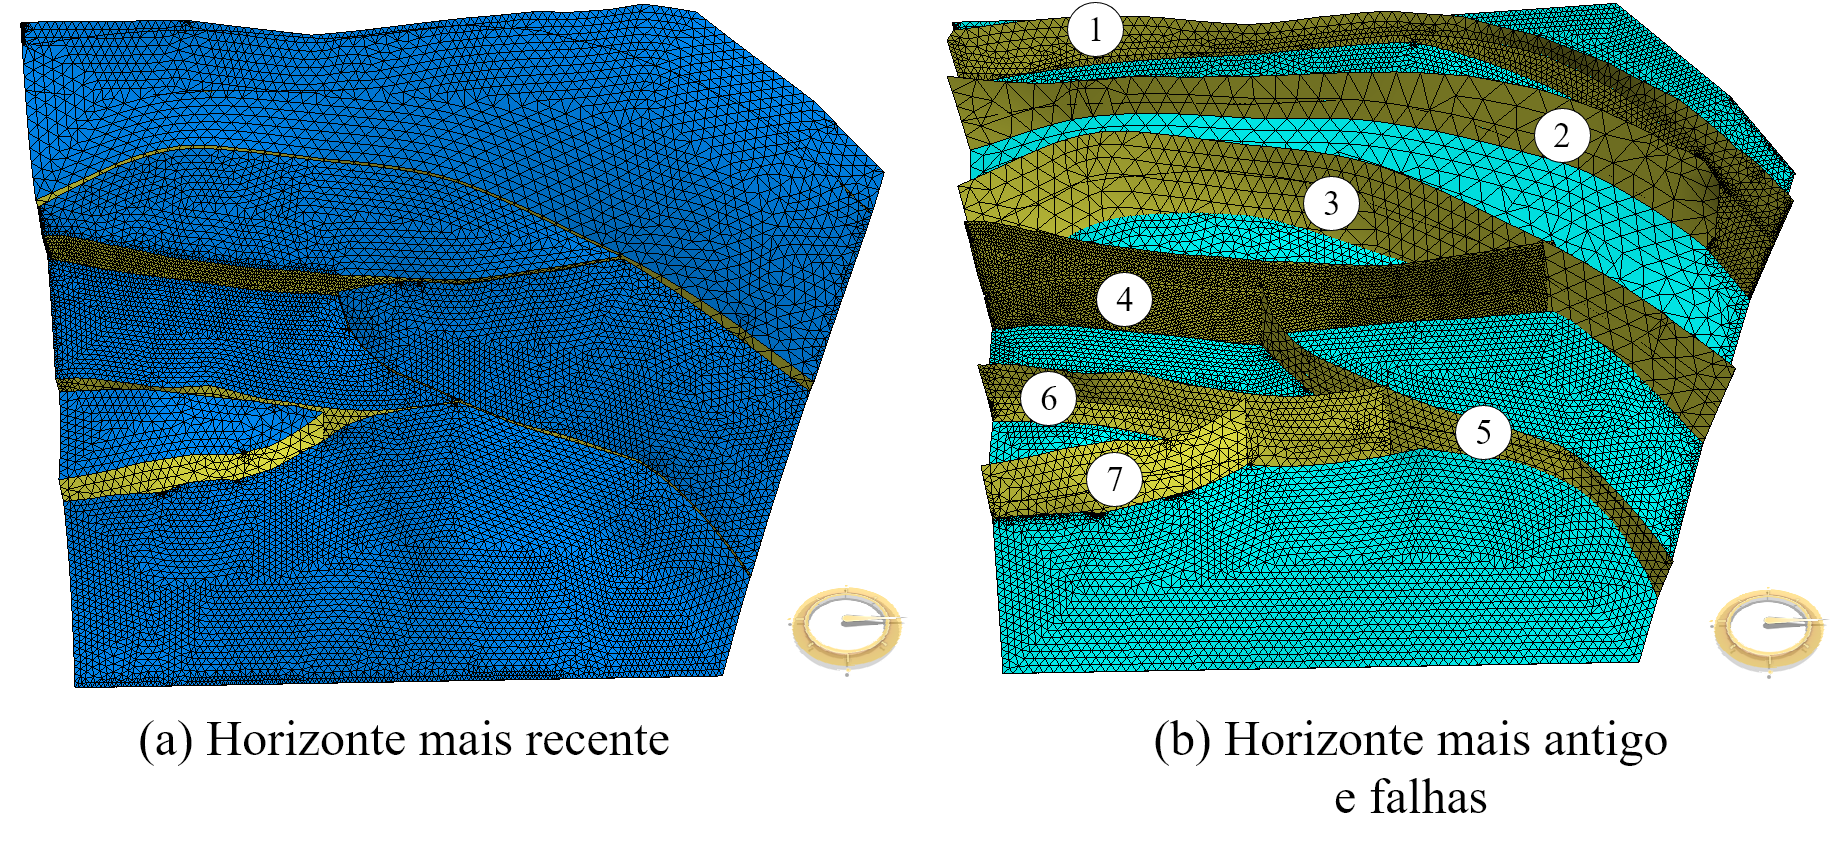
\includegraphics[width=\textwidth]{images/fig-example-2-1}
    \caption{Vista de cima do modelo geológico adaptado cedido pelo Cenpes.}\label{fig-example-2-1}
  \end{center}
\end{figure}



\begin{figure} [H]
  \begin{center}
    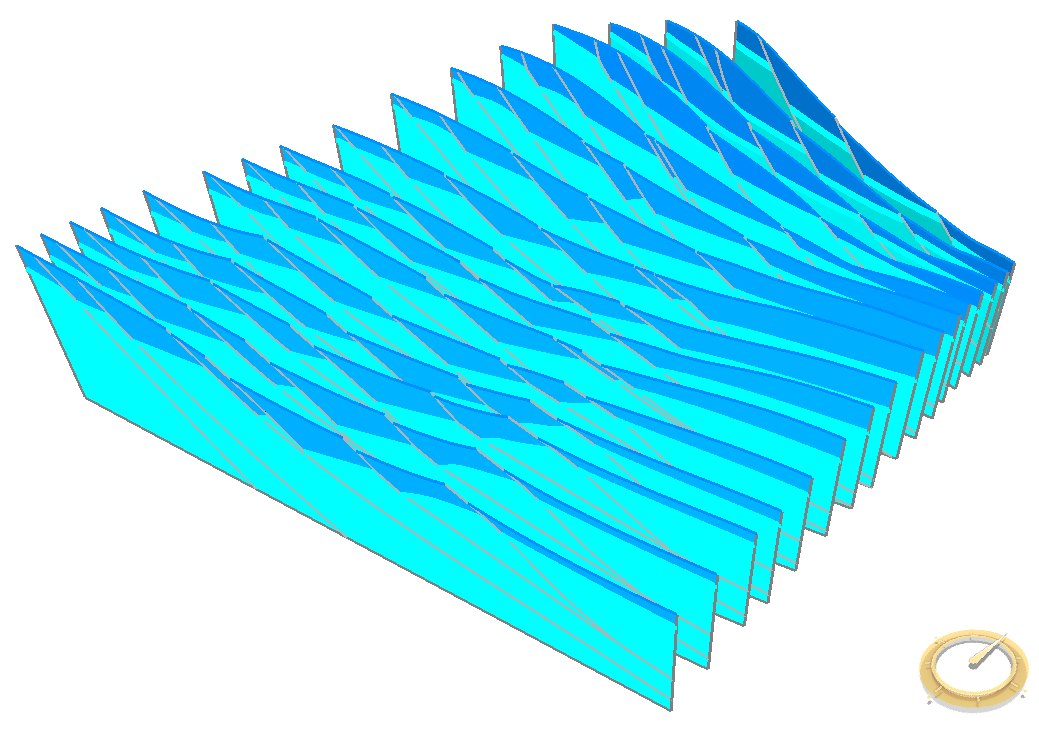
\includegraphics[width=320pt]{images/fig-example-2-2}
    \caption{Vista das seções que compõem o modelo geológico adaptado cedido pelo Cenpes.}\label{fig-example-2-2}
  \end{center}
\end{figure}

Conforme mencionado, a primeira ação para iniciar o mapeamento de superfícies é a criação das \textit{LMModels} a partir das seções geológicas restauradas e após isso criar a estrutura de dados como apresentado na Figura~\ref{fig-lmm-data-structure}. As \textit{LMModels} das seções no ambiente multisseção do Sistema Recon são apresentadas na Figura~\ref{fig-example-2-3}.

\begin{figure} [H]
  \begin{center}
    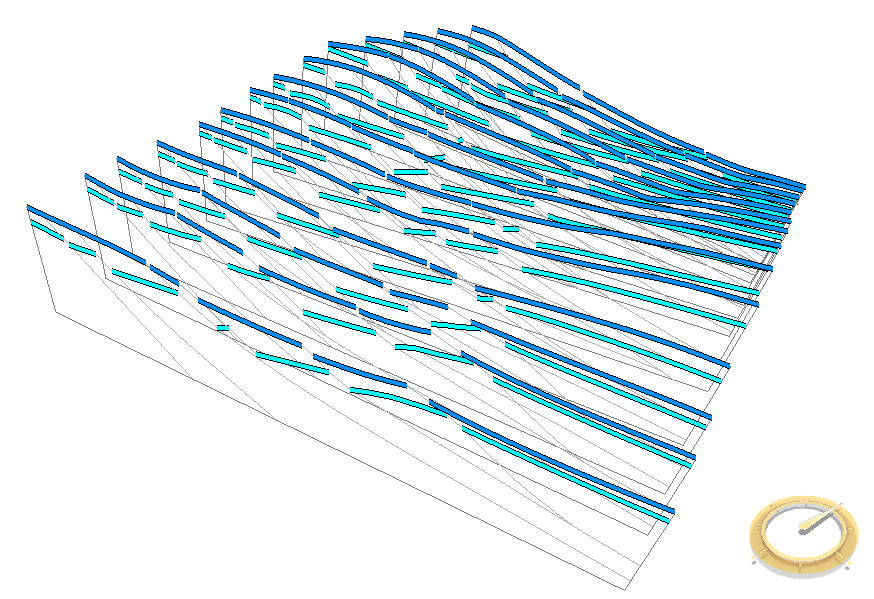
\includegraphics[width=320pt]{images/fig-lmmodel-ms}
    \caption{Vista das \textit{LMModels} do modelo geológico adaptado cedido pelo Cenpes.}.\label{fig-example-2-3}
  \end{center}
\end{figure}

Com as \textit{LMModels} criadas, parte-se então para o \textit{remesh} das malhas das superfícies para inclusão dos nós das \textit{LMModels} da primeira \textit{EtapaMS}. Conforme já visto, a regeração das malhas de superfícies com os pontos da \textit{LMModels} é importante para que haja uma ligação direta com o que ocorre nas seções e assim ter a principal base de dados vindos da seção para o mapeamento de superfícies. A nova malha da superfície do topo é mostrada na Figura~\ref{fig-example-2-4} juntamente das \textit{LMModels}.

\begin{figure} [h]
  \begin{center}
    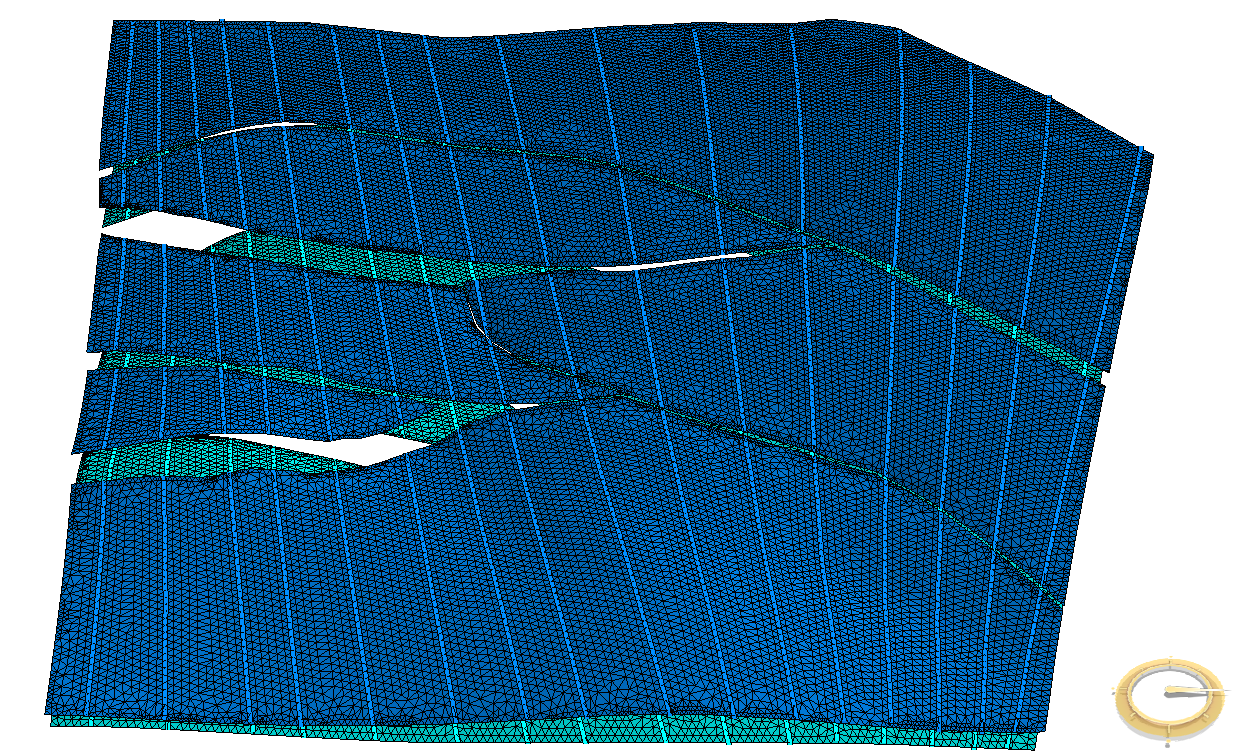
\includegraphics[width=\textwidth]{images/fig-example-2-3}
    \caption{Visão geral da nova malha de superfície do modelo geológico adaptado cedido pelo Cenpes.}\label{fig-example-2-4}
  \end{center}
\end{figure}

A primeira \textit{EtapaMS} possui os cenários das seções que restauram a falha 7, que são um total de 6 seções, como mostra a Figura~\ref{fig-example-2-5}. Nesta \textit{EtapaMS} apenas as seções que cortam a falha 7 se movimentam. Essa forma de organizar as cenários que realizam a mesma atividade em uma \textit{EtapaMS} é muito importante para o mapeamento de superfícies, pois favorece um comportamento coerente com a movimentação tectônica quando se deforma a superfície.

\begin{figure} [H]
  \begin{center}
    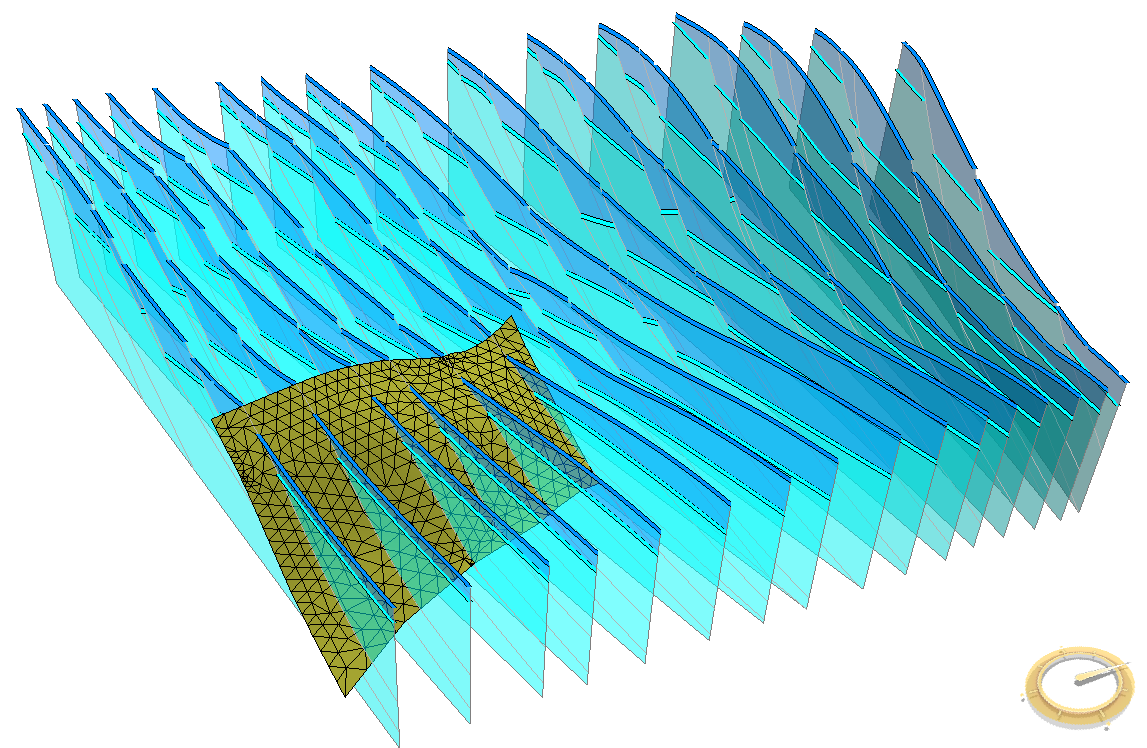
\includegraphics[width=300pt]{images/fig-example-2-5}
    \caption{Falha 7 do modelo em destaque na \textit{EtapaMS} inicial.}\label{fig-example-2-5}
  \end{center}
\end{figure}

Com a primeira falha já definida, é possível passar para a fase de seleção das bordas origem e destino na superfície do topo. São selecionados trechos de bordas de pedaços diferentes da superfície, pois a falha 7 está entre tais pedaços. As bordas origem e destino dessa primeira \textit{EtapaMS} podem ser vistas na Figura~\ref{fig-example-2-6}.

\begin{figure} [H]
  \begin{center}
    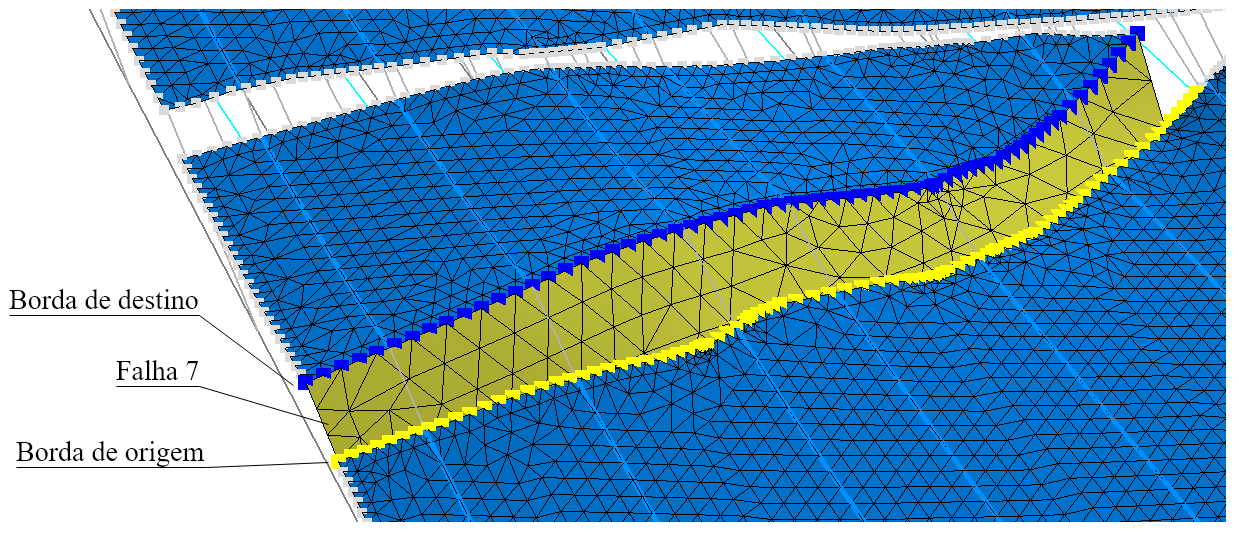
\includegraphics[width=350pt]{images/fig-example-2-6}
    \caption{Bordas origem e destino da \textit{EtapaMS} referente à falha 7.}\label{fig-example-2-6}
  \end{center}
\end{figure}

Conforme apresentado anteriormente, a fase seguinte é o cálculo dos pontos destino dos nós da borda de origem. Faz-se a definição, para cada ponto da superfície, do atributo \quotes{move} ou \quotes{não move}. Após isso pode-se executar o deformador de superfícies e o resultado (antes e depois) pode ser conferido na Figura~\ref{fig-example-2-7}.

\begin{figure} [H]
  \begin{center}
    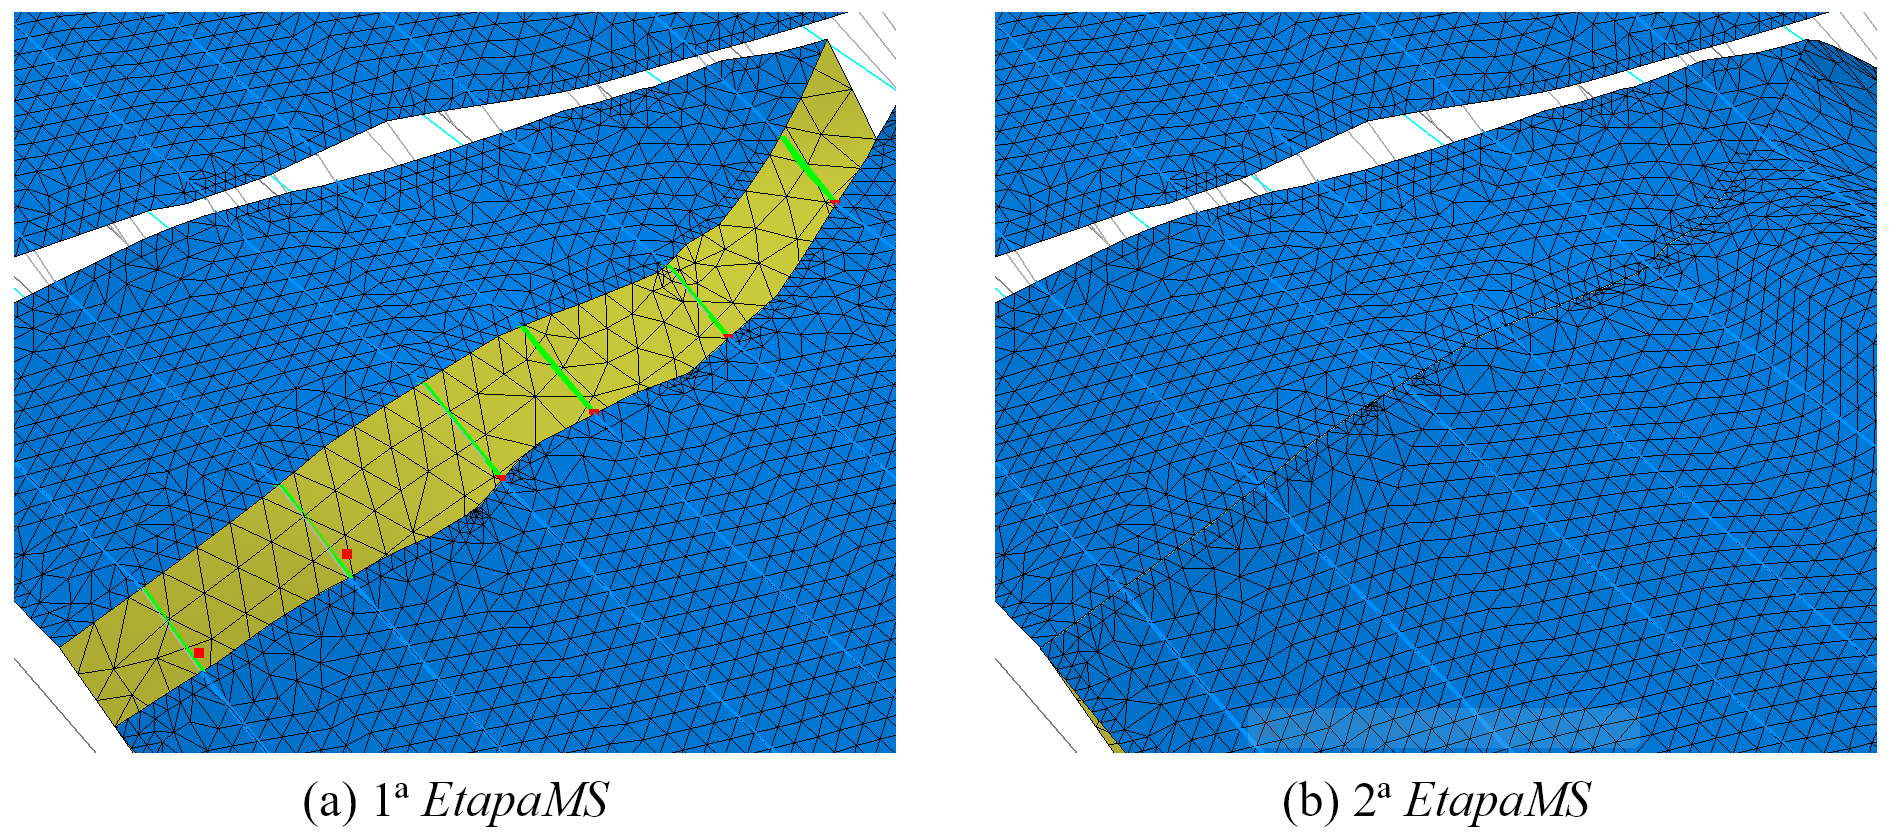
\includegraphics[width=\textwidth]{images/fig-example-2-7}
    \caption{Antes e depois da execução do deformador na superfície do topo na \textit{EtapaMS} inicial.}\label{fig-example-2-7}
  \end{center}
\end{figure}

Para a superfície mais antiga, também é chamado o deformador mas sem uma definição de bordas origem e destino, ficando restrita apenas aos pontos de controle das \textit{LMModels}. Na ilustração do antes e depois dessa superfície (Figura~\ref{fig-example-2-8}) é notável que a parte que se move não chega a coincidir com o pedaço imóvel nesta \textit{EtapaMS}, no entanto, é isso que também ocorre na restauração das seções, o que evidencia o caráter de conformidade desse mapeamento com o que acontece nas seções.

\begin{figure} [H]
  \begin{center}
    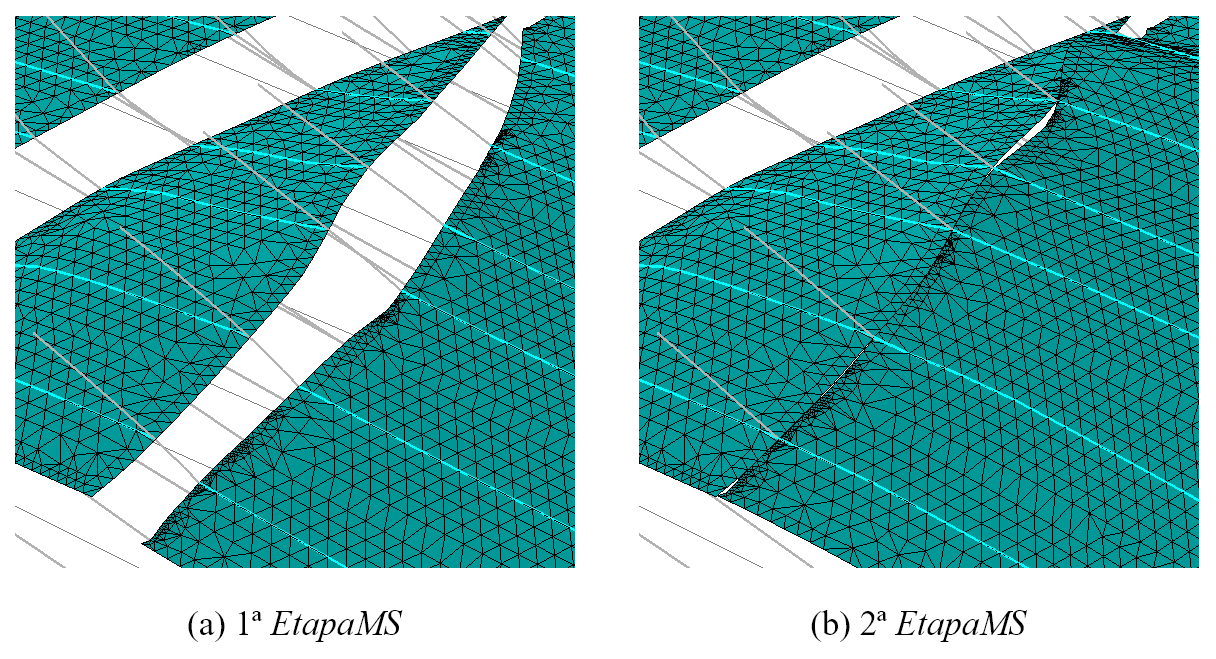
\includegraphics[width=340pt]{images/fig-example-2-8}
    \caption{Antes e depois da execução do deformador na superfície mais antiga na \textit{EtapaMS} inicial.}\label{fig-example-2-8}
  \end{center}
\end{figure}

Esse processo é repetido para cada uma das \textit{EtapasMS} do modelo, onde sempre um novo trecho de bordas origem e destino precisa ser definido (exceto em \textit{EtapaMS} de descompactação). A sequência das Figuras~\ref{fig-example-2-9} até \ref{fig-example-2-12} destaca cada um dos mapeamentos feitos com sua respectiva \textit{EtapaMS}:

\begin{figure} [H]
  \begin{center}
    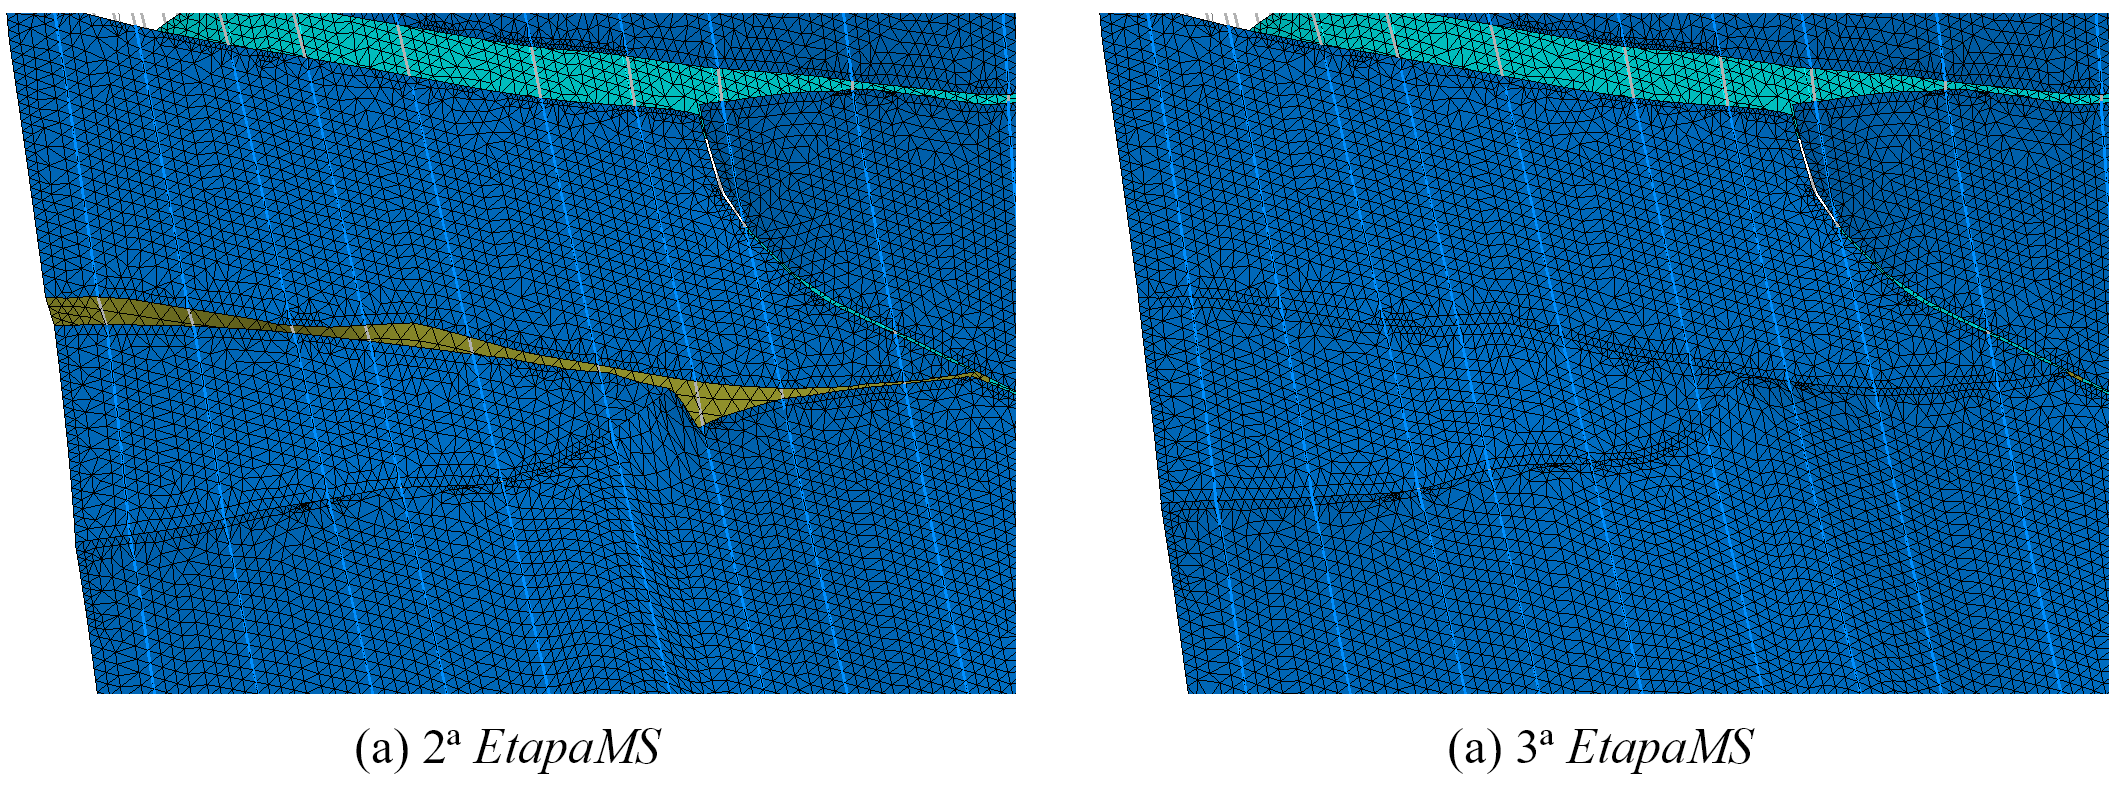
\includegraphics[width=\textwidth]{images/fig-example-2-9}
    \caption{Mapeamento da superfície conforme as seções da 2ª \textit{EtapaMS} (falha 6).}\label{fig-example-2-9}
  \end{center}
\end{figure}

\begin{figure} [H]
  \begin{center}
    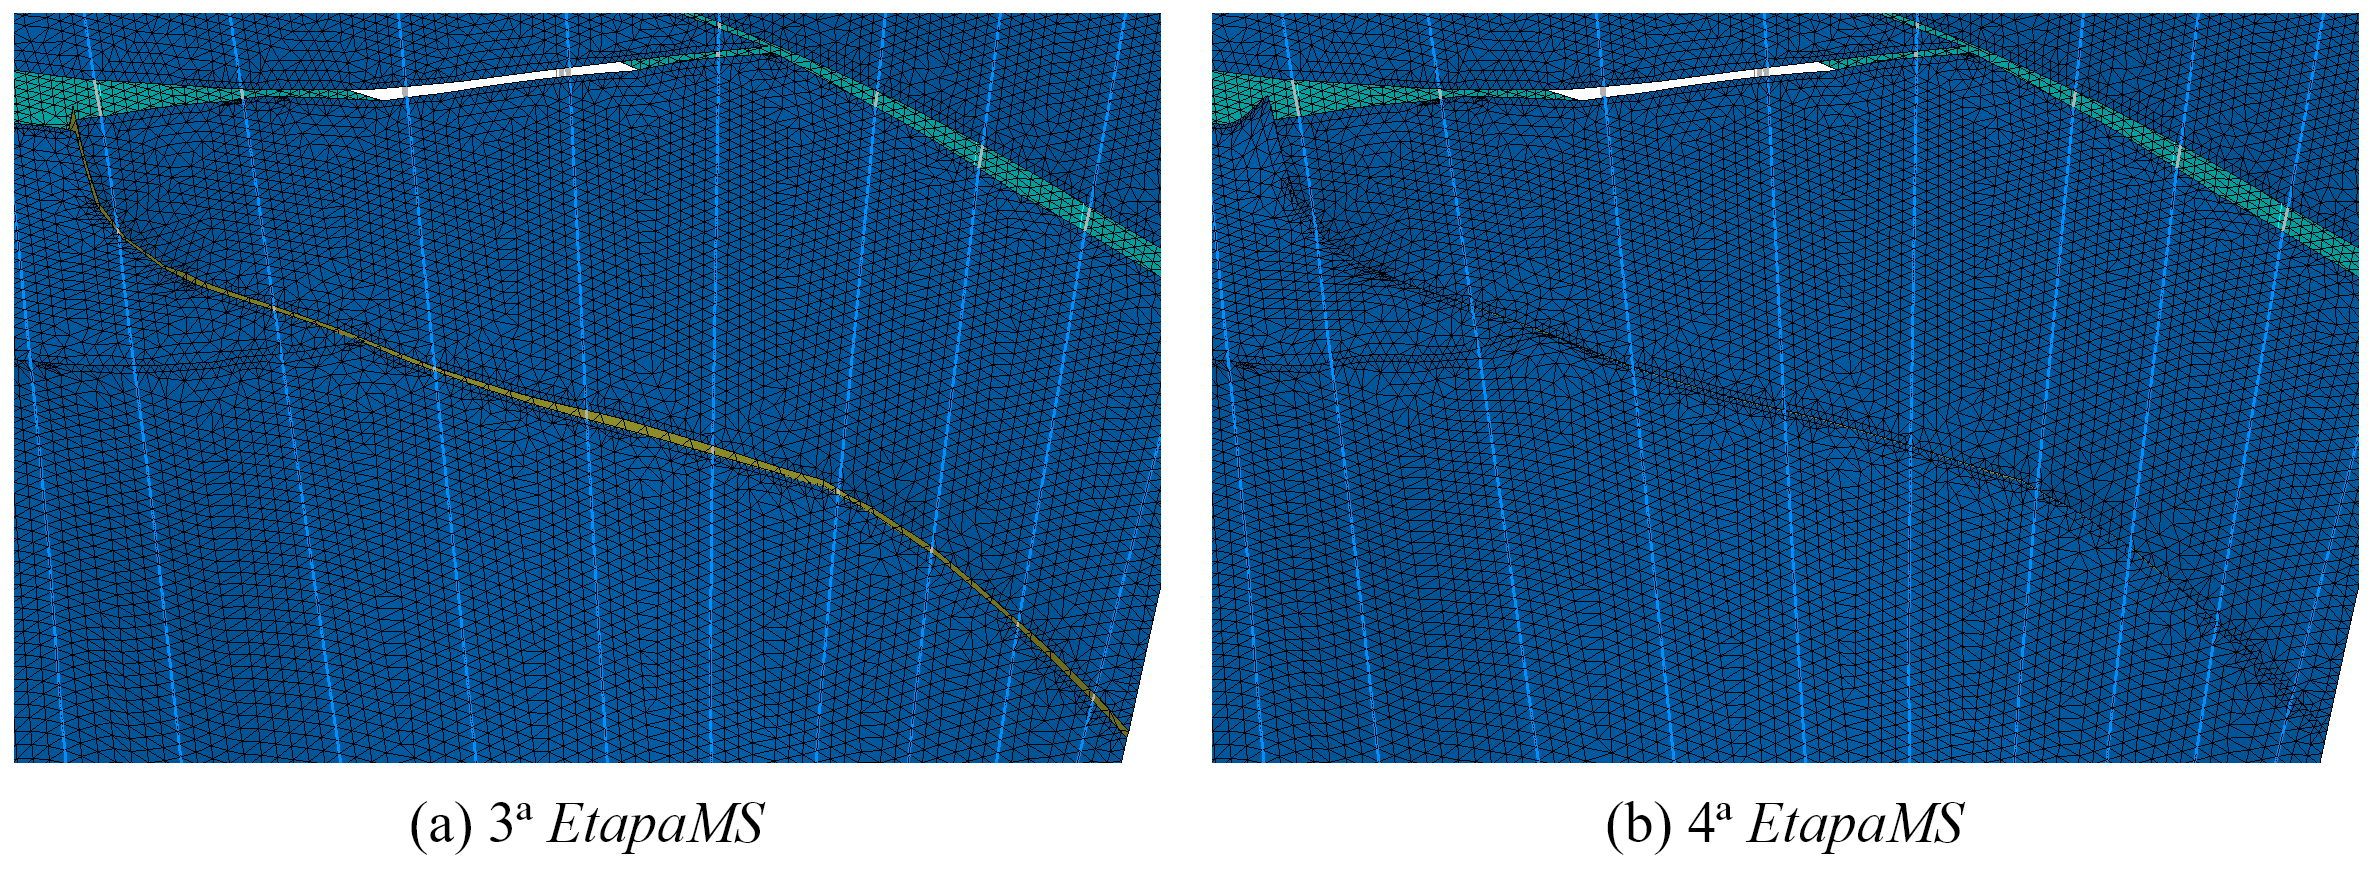
\includegraphics[width=\textwidth]{images/fig-example-2-10}
    \caption{Mapeamento da superfície conforme as seções da 3ª \textit{EtapaMS} (falha 5).}\label{fig-example-2-10}
  \end{center}
\end{figure}

\begin{figure} [H]
  \begin{center}
    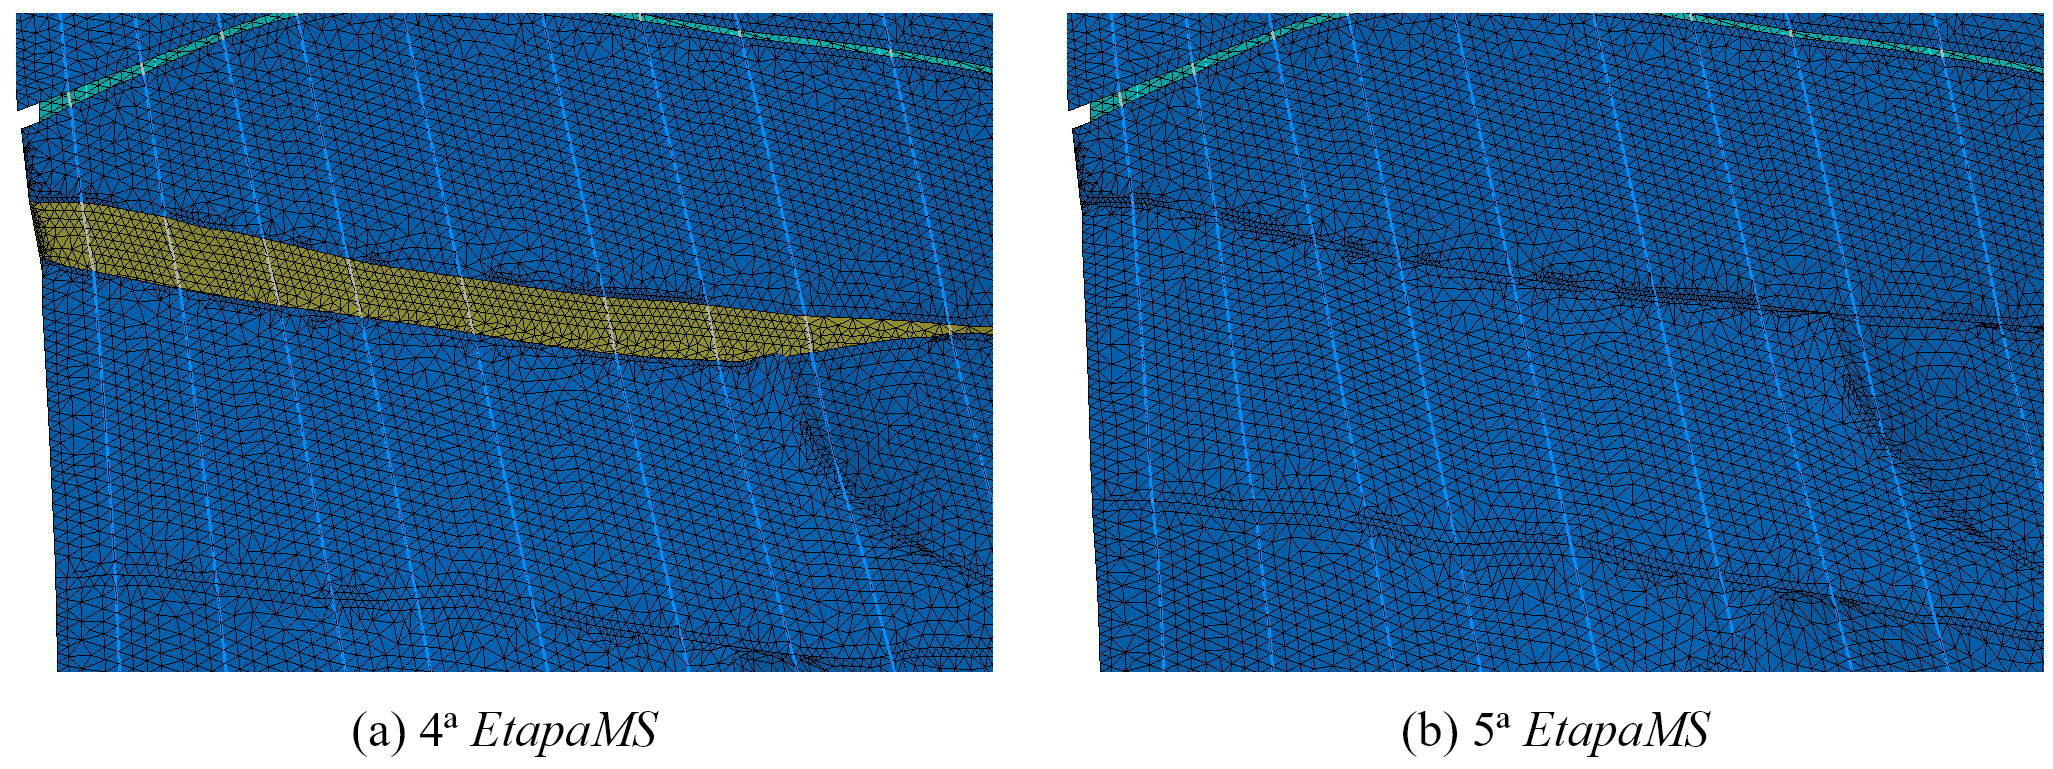
\includegraphics[width=\textwidth]{images/fig-example-2-11}
    \caption{Mapeamento da superfície conforme as seções da 4ª \textit{EtapaMS} (falha 4).}\label{fig-example-2-11}
  \end{center}
\end{figure}

\begin{figure} [H]
  \begin{center}
    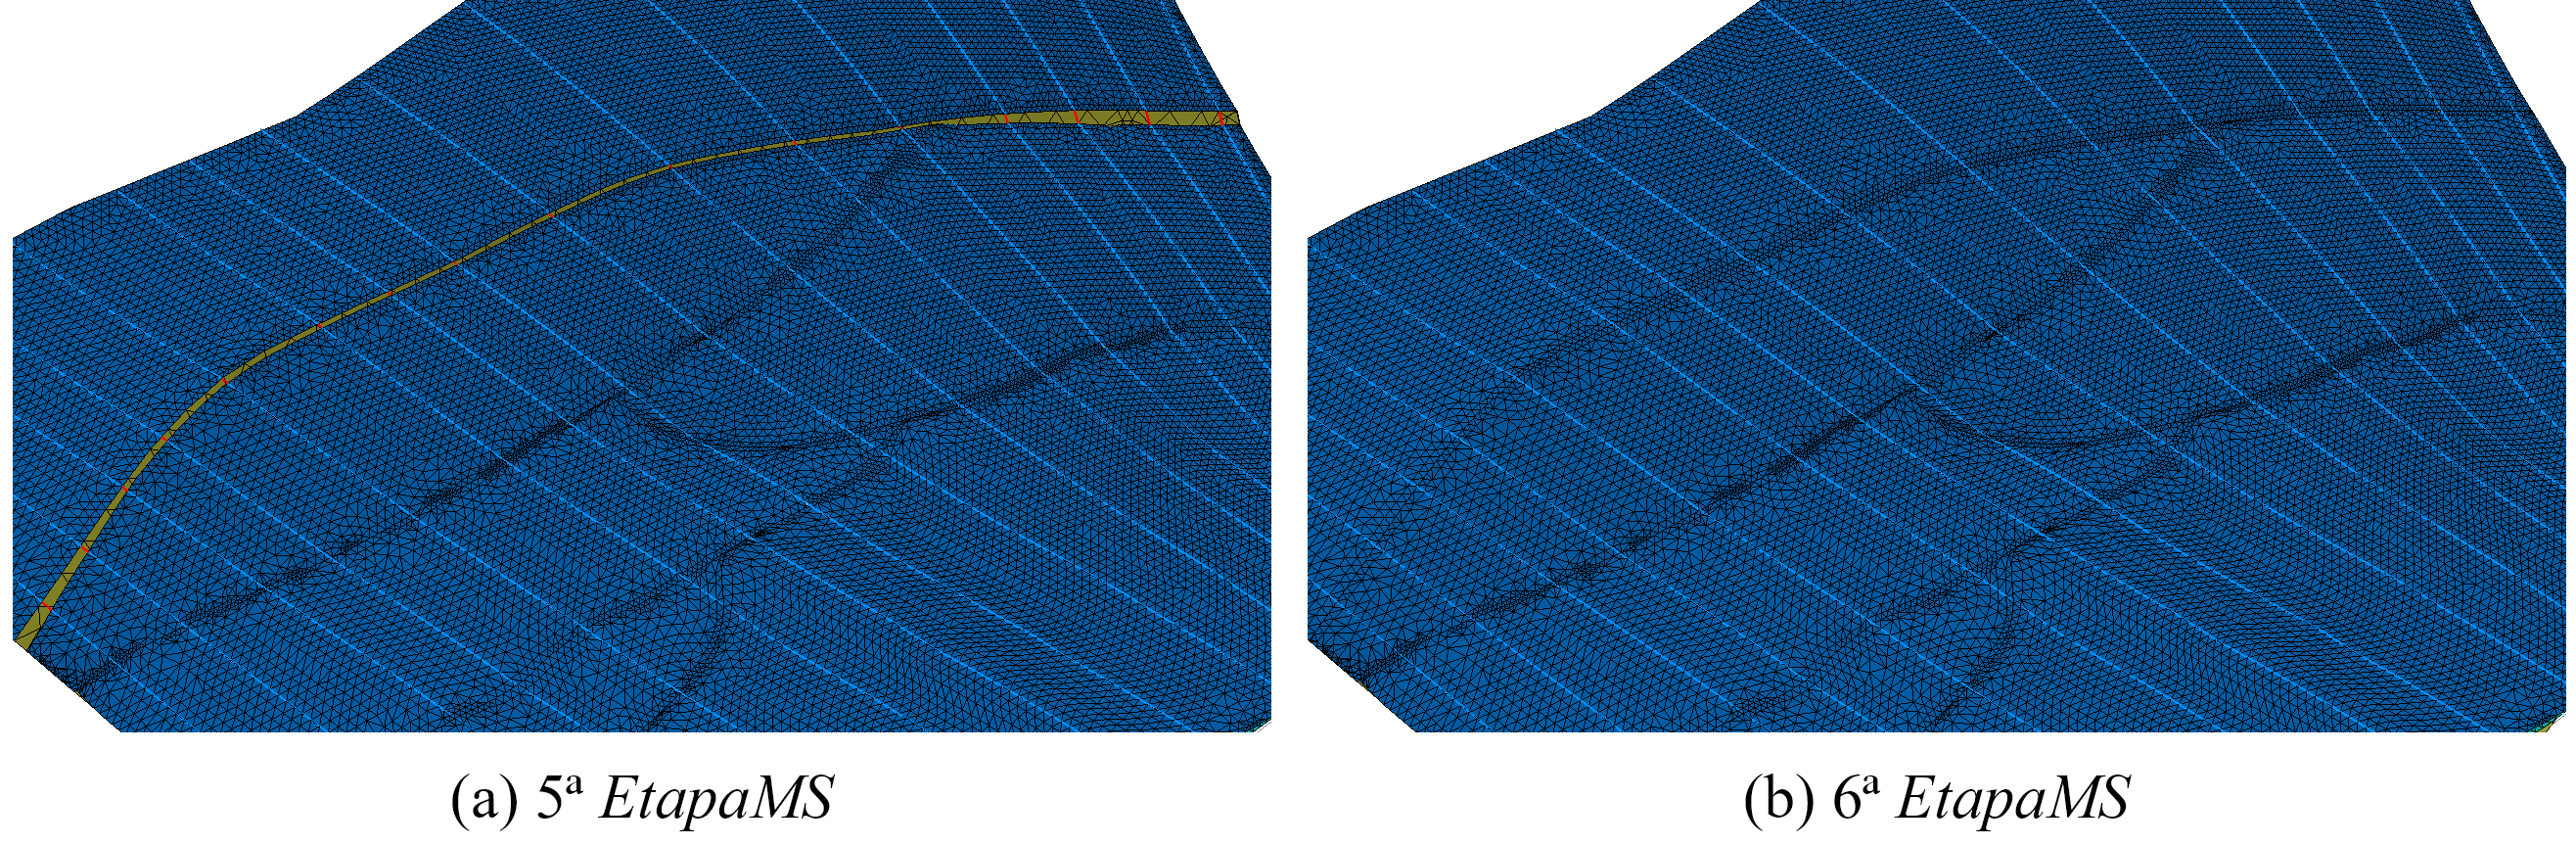
\includegraphics[width=\textwidth]{images/fig-example-2-12}
    \caption{Mapeamento da superfície conforme as seções da 5ª \textit{EtapaMS} (falha 3).}\label{fig-example-2-12}
  \end{center}
\end{figure}

A \textit{EtapaMS} seguinte seria com a ocorrência de uma descompactação da camada do topo, o que \quotes{alivia} a camada de baixo fazendo com que haja um soerguimento do horizonte mais antigo. Para o mapeamento, as \textit{LMModels} irão trazer essa informação e, consequentemente, todos os pontos sofrerão um deslocamento, logo, todos os nós da superfície de baixo serão marcados como \quotes{move}. Daí em diante, repete-se o processo de escolha de bordas conforme a falha da \textit{EtapaMS} corrente, com a diferença de que agora apenas a superfície de baixo existirá no modelo.

Uma última ilustração do mapeamento de superfícies nesse modelo pode ser vista na Figura~\ref{fig-example-2-13} sob um ponto de vista global.

\begin{figure} [H]
  \begin{center}
    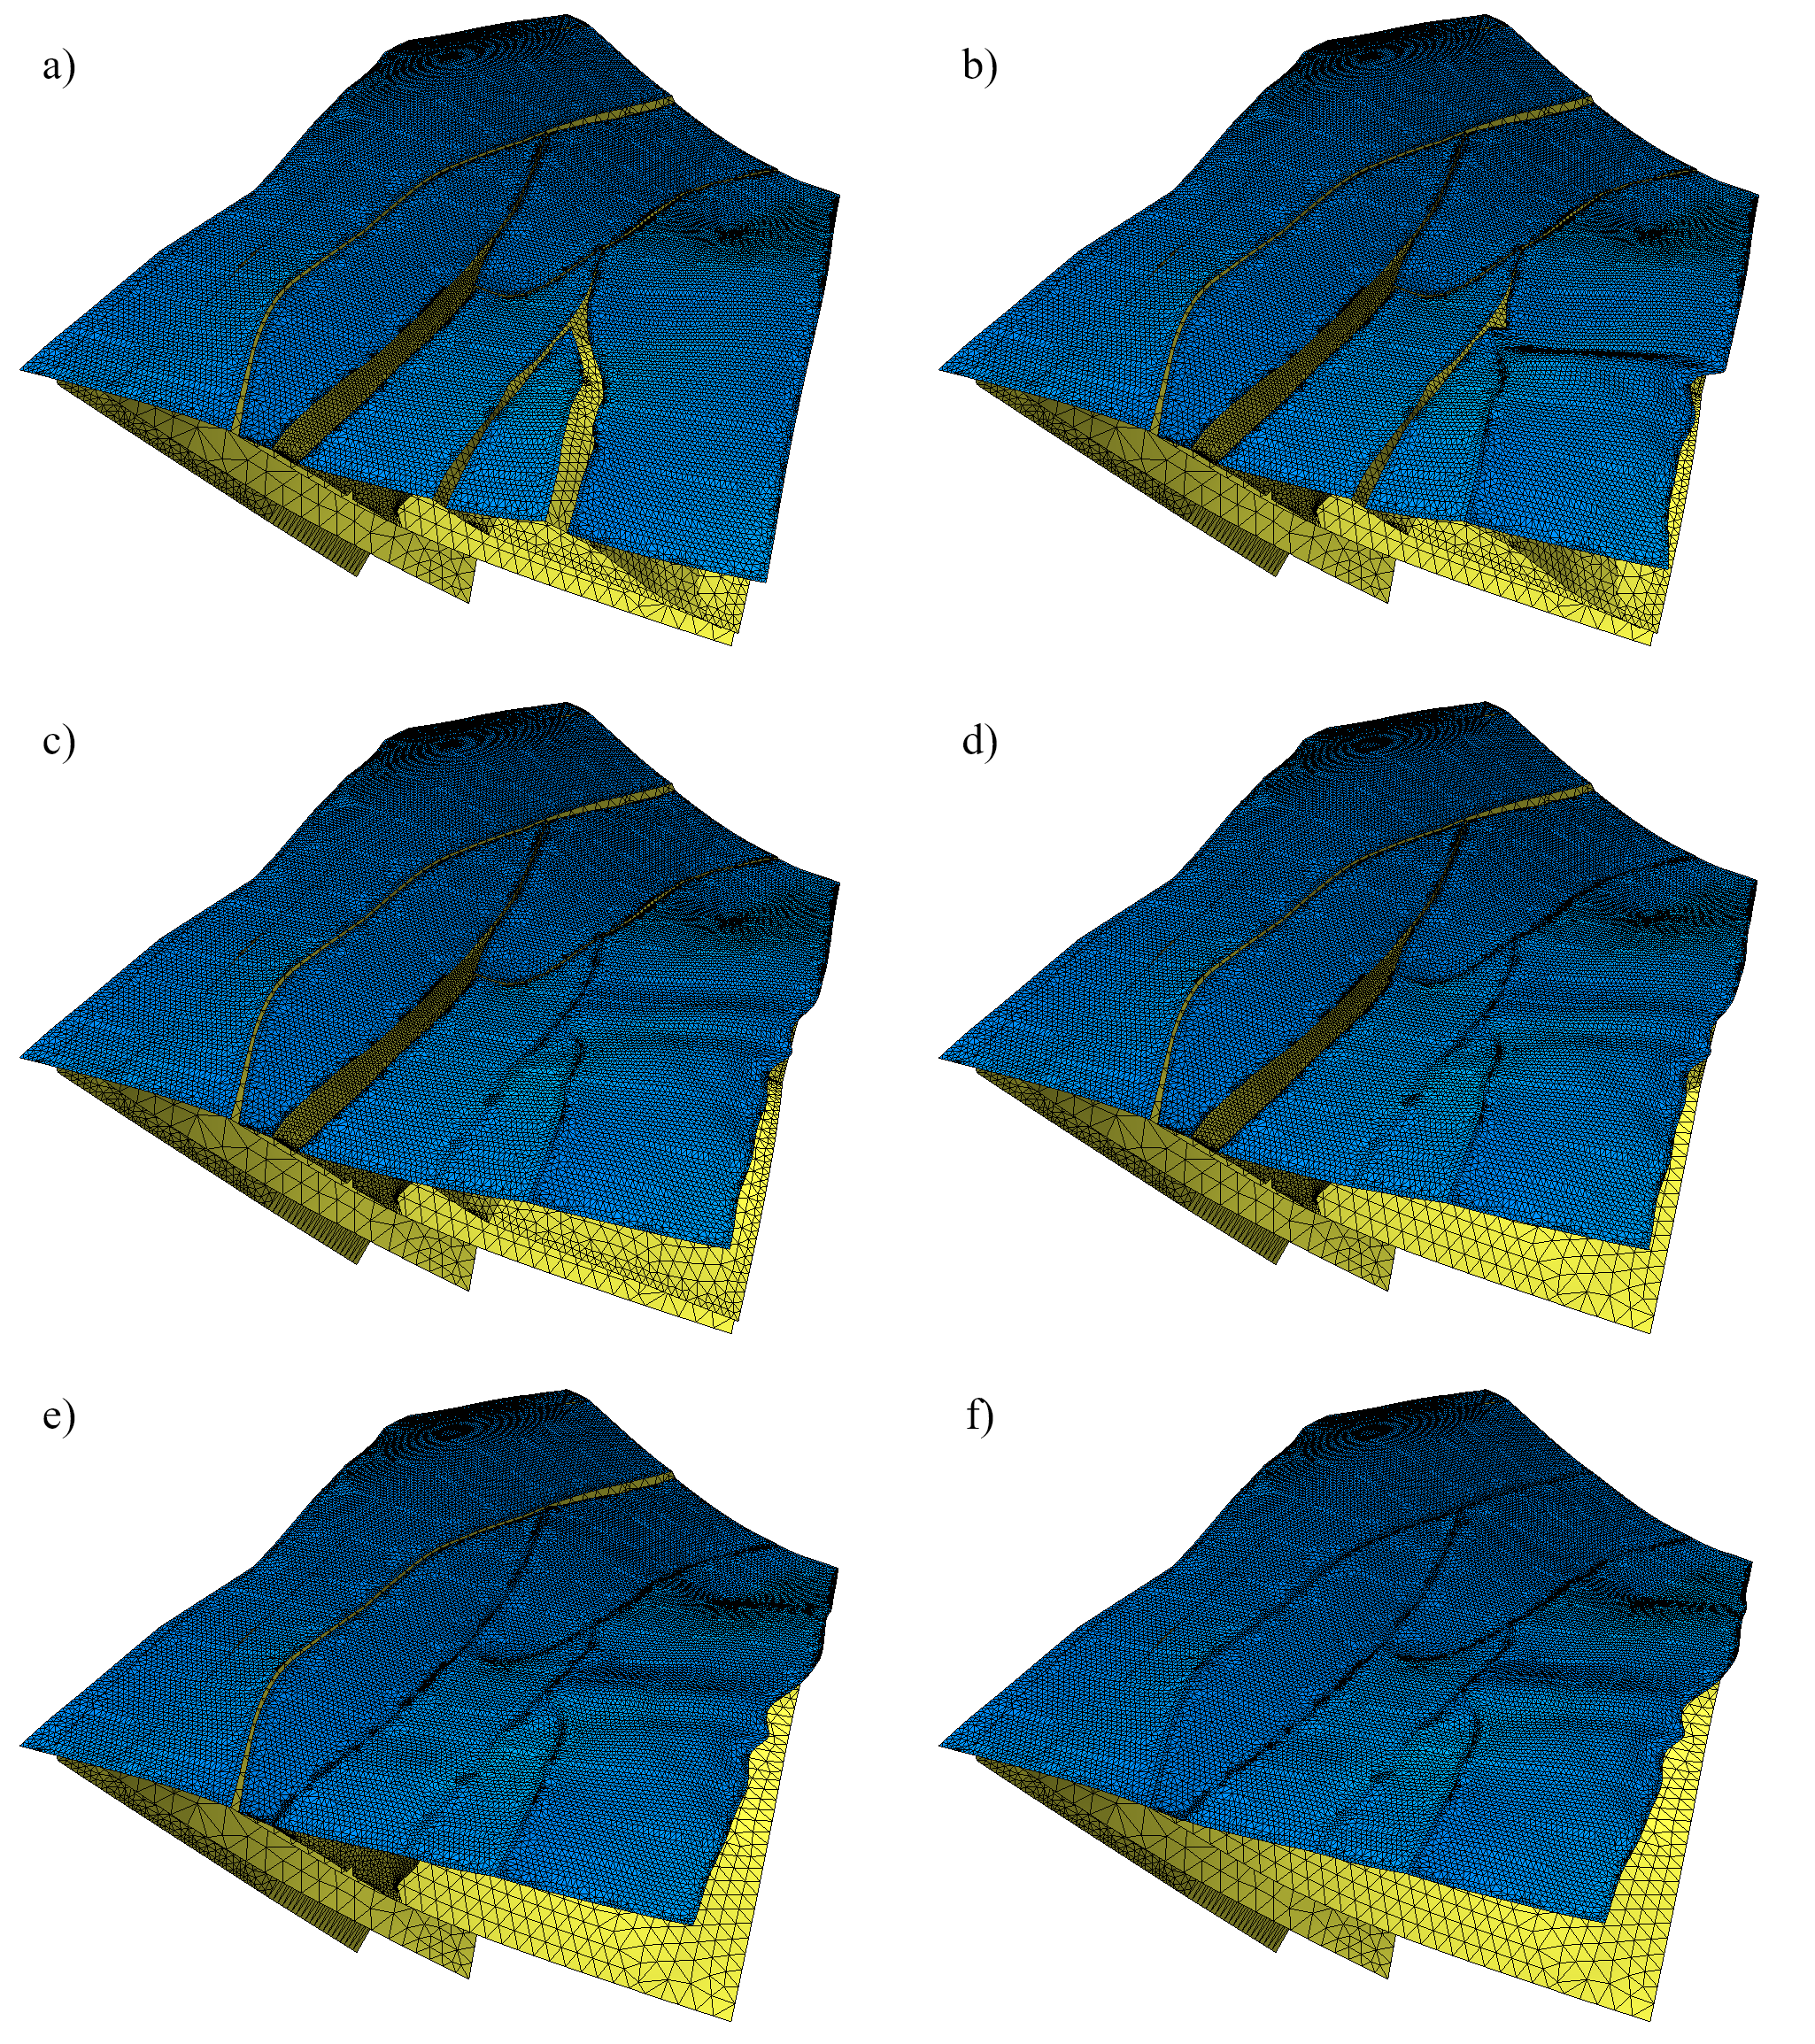
\includegraphics[width=\textwidth]{images/fig-example-2-13}
    \caption{Mapeamento da superfície do modelo.(a) Etapa inicial, (b) falha 7, (c) falha 6, (d) falha 5, (e) falha 4 e (f) falha 5.}\label{fig-example-2-13}
  \end{center}
\end{figure}

Pela visualização do que acontece com as superfícies de horizonte se deformando a cada passo do conjunto de movimentações ocorrido nas seções, pode-se induzir que este processo, aqui chamado de mapeamento de superfícies, poderia ser nomeado de restauração de superfícies e uma breve discussão a respeito desses termos pode ser conferida no capítulo de conclusão deste trabalho.


